\documentclass{beamer}
\usepackage{amsmath,amssymb,amsthm}
\usepackage{algorithm,algorithmic}

\usepackage{tikz}
\usetikzlibrary{arrows,shapes,chains,matrix,positioning,scopes,patterns}
\usepackage{pgfplots}
\usepgflibrary{shapes}
\pgfplotsset{compat=1.6}

\usetheme{default}
\setbeamertemplate{navigation symbols}{\textcolor{blue}{\insertframenumber / \inserttotalframenumber}}

\newcommand{\expt}{\mathbb{E}}
\newcommand{\indicator}[1]{\mathbbm{1}_{\left\{ {#1} \right\} }}
\newcommand{\abs}[1]{\left\lvert#1\right\rvert}

\newlength\tikzwidth
\newlength\tikzheight

\title{\large{Spatially-Coupled Codes for Side-Information Problems}}
\author{\normalsize{\textbf{Santhosh Kumar} \\ Avinash Vem \\ Krishna Narayanan \\ Henry Pfister}}
\date{June 30, 2014}

\begin{document}

\begin{frame}
  \titlepage
\end{frame}

\begin{frame}{Lossy Source Coding Problem}
  \centering{$X^n=(X_1,\cdots,X_n)$, $\alert{X_i \sim \mathsf{Bernoulli}(\frac{1}{2})}$ \\ \vspace{0.3cm} \alert{Binary code $\mathcal{C}=(n,k)$}, rate $R=k/n$}
  \begin{block}{Lossy Source Coding}<2->
    \begin{columns}
      \column{0.55\textwidth}
      \begin{itemize}
      \item<2-> Compress $X^n$ to $\hat{X}^n \in \mathcal{C}$
      \item<2-> \textcolor{blue}{Min.~Hamming distortion}
        \begin{align*}
          D=\frac{1}{n} \sum_{i=1}^n \expt \abs{X_i-\hat{X}_i}
        \end{align*}
      \item<3-> Rate-Distortion theory: \vspace{-0.15cm}
        \begin{align*}
          R > 1 - h(D)
        \end{align*}
        \vspace{-0.5cm}
      \item<3-> $h(\cdot)$ is binary entropy function
        \small{
          \begin{align*}
            h(D)\!=\!-D \log_2 D \!-\! (1\!-\!D) \log_2 (1-D)
          \end{align*}
        }
      \end{itemize}
      \column{0.45\textwidth}<3->
      \setlength\tikzheight{3cm} 
      \setlength\tikzwidth{3.5cm} 
      \centering{\begin{tikzpicture}
  \begin{axis}[%
    font=\small,
    scale only axis,
    width=\tikzwidth,
    height=\tikzheight,
    xmin=0, xmax=0.5,
    ymin=0, ymax=1,
    xlabel={Distortion $D$},
    ylabel={Rate $R$},
    xmajorgrids,
    ymajorgrids]

    \filldraw[fill=black!30,draw=black]
    (axis description cs:0.0000,1.0000) -- 
    (axis description cs:0.0200,0.9192) -- 
    (axis description cs:0.0400,0.8586) -- 
    (axis description cs:0.0600,0.8056) -- 
    (axis description cs:0.0800,0.7577) -- 
    (axis description cs:0.1000,0.7136) -- 
    (axis description cs:0.1200,0.6726) -- 
    (axis description cs:0.1400,0.6341) -- 
    (axis description cs:0.1600,0.5978) -- 
    (axis description cs:0.1800,0.5635) -- 
    (axis description cs:0.2000,0.5310) -- 
    (axis description cs:0.2200,0.5001) -- 
    (axis description cs:0.2400,0.4706) -- 
    (axis description cs:0.2600,0.4426) -- 
    (axis description cs:0.2800,0.4158) -- 
    (axis description cs:0.3000,0.3902) -- 
    (axis description cs:0.3200,0.3657) -- 
    (axis description cs:0.3400,0.3423) -- 
    (axis description cs:0.3600,0.3199) -- 
    (axis description cs:0.3800,0.2985) -- 
    (axis description cs:0.4000,0.2781) -- 
    (axis description cs:0.4200,0.2585) -- 
    (axis description cs:0.4400,0.2398) -- 
    (axis description cs:0.4600,0.2220) -- 
    (axis description cs:0.4800,0.2050) -- 
    (axis description cs:0.5000,0.1887) -- 
    (axis description cs:0.5200,0.1733) -- 
    (axis description cs:0.5400,0.1585) -- 
    (axis description cs:0.5600,0.1445) -- 
    (axis description cs:0.5800,0.1313) -- 
    (axis description cs:0.6000,0.1187) -- 
    (axis description cs:0.6200,0.1068) -- 
    (axis description cs:0.6400,0.0956) -- 
    (axis description cs:0.6600,0.0851) -- 
    (axis description cs:0.6800,0.0752) -- 
    (axis description cs:0.7000,0.0659) -- 
    (axis description cs:0.7200,0.0573) -- 
    (axis description cs:0.7400,0.0493) -- 
    (axis description cs:0.7600,0.0420) -- 
    (axis description cs:0.7800,0.0352) -- 
    (axis description cs:0.8000,0.0290) -- 
    (axis description cs:0.8200,0.0235) -- 
    (axis description cs:0.8400,0.0185) -- 
    (axis description cs:0.8600,0.0142) -- 
    (axis description cs:0.8800,0.0104) -- 
    (axis description cs:0.9000,0.0072) -- 
    (axis description cs:0.9200,0.0046) -- 
    (axis description cs:0.9400,0.0026) -- 
    (axis description cs:0.9600,0.0012) -- 
    (axis description cs:0.9800,0.0003) -- 
    (axis description cs:1.0000,0.0000) -- 
    (axis description cs:1.0000,1.0000) -- cycle;
    
    \node at (axis description cs:0.6000,0.5000) {$R>1-h(D)$};
  \end{axis}
\end{tikzpicture}}
    \end{columns}
  \end{block}

\end{frame}

\begin{frame}{Side-Information Problems: Wyner-Ziv}
  \begin{center}
    \scalebox{0.5}{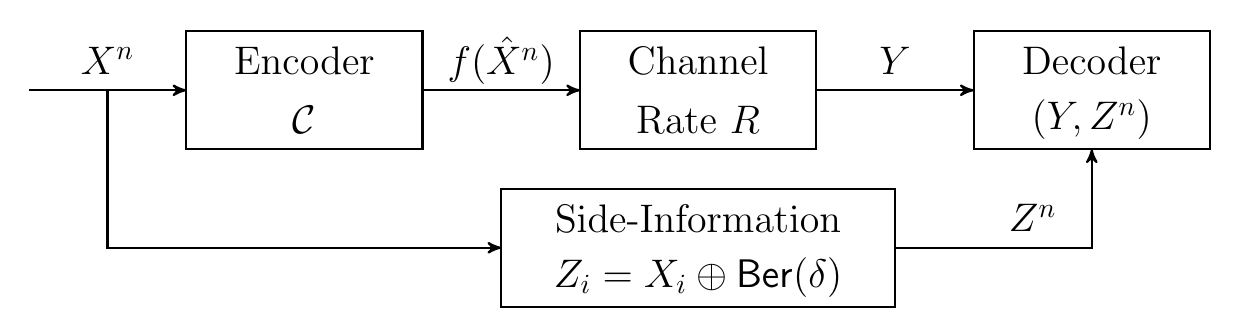
\begin{tikzpicture}
  [node distance=1cm,draw=black,thick, >=stealth']

  \def \reclen {3}
  \def \linelen {2}
  \def \recwid {0.75}

  \draw[->] (0,0) -- (0+\linelen,0);
  \draw (0+\linelen,\recwid) rectangle (0+\linelen+\reclen,-\recwid);
  \draw[->] (0+\linelen+\reclen,0) -- (0+\linelen+\reclen+\linelen,0);
  \draw (0+\linelen+\reclen+\linelen,\recwid) rectangle (0+\linelen+\reclen+\linelen+\reclen,-\recwid);
  \draw[->] (0+\linelen+\reclen+\linelen+\reclen,0) -- (0+\linelen+\reclen+\linelen+\reclen+\linelen,0);
  \draw (0+\linelen+\reclen+\linelen+\reclen+\linelen,\recwid) rectangle (0+\linelen+\reclen+\linelen+\reclen+\linelen+\reclen,-\recwid);

  \draw[->] (0.5*\linelen,0) -- (0.5*\linelen,-2) -- (1.5*\linelen+\reclen,-2);
  \draw (1.5*\linelen+\reclen,-2+\recwid) rectangle (2.5*\linelen+2*\reclen,-2-\recwid);
  \draw[->] (2.5*\linelen+2*\reclen,-2) -- (2*\linelen+2*\reclen+\linelen+0.5*\reclen,-2) -- (2*\linelen+2*\reclen+\linelen+0.5*\reclen,-\recwid);

  \node at (\linelen+0.5*\reclen,0.5*\recwid) {\Large{Encoder}};
  \node at (\linelen+0.5*\reclen,-0.5*\recwid) {\Large{$\mathcal{C}$}};

  \node at (2*\linelen+1.5*\reclen,0.5*\recwid) {\Large{Channel}};
  \node at (2*\linelen+1.5*\reclen,-0.5*\recwid) {\Large{Rate $R$}};

  \node at (3*\linelen+2.5*\reclen,0.5*\recwid) {\Large{Decoder}};
  \node at (3*\linelen+2.5*\reclen,-0.5*\recwid) {\Large{$(Y,Z^n)$}};

  \node at (2*\linelen+1.5*\reclen,-2+0.5*\recwid) {\Large{Side-Information}};
  \node at (2*\linelen+1.5*\reclen,-2-0.5*\recwid) {\Large{$Z_i=X_i\oplus \mathsf{Ber}(\delta)$}};

  \node at (0.5*\linelen,0.5*\recwid) {\Large{$X^n$}};
  \node at (1.5*\linelen+\reclen,0.5*\recwid) {\Large{$f(\hat{X}^n)$}};
  \node at (2.5*\linelen+2*\reclen,0.5*\recwid) {\Large{$Y$}};
  \node at (3*\linelen+2.25*\reclen,-2+0.5*\recwid) {\Large{$Z^n$}};

\end{tikzpicture}

%%% Local Variables: 
%%% mode: latex
%%% TeX-master: "../talk"
%%% End: 
}
  \end{center}
  \begin{block}{Wyner-Ziv Formulation}<1->
    \begin{columns}
      \column{0.55\textwidth}
      \begin{itemize}
      \item<1-> \textcolor{red}{Side-information} $Z^n$ about $X^n$
      \item<1-> Decoder \textcolor{blue}{additionally} has $Z^n$
      \item<1-> Say $Z_i = X_i \oplus \mathsf{Ber}(\delta)$
      \item<2-> Wyner-Ziv theory:
        \begin{align*}
          R > l.c.e\{h(D*\delta)-h(D), (\delta,0)\}
        \end{align*}
      \item<2-> $D*\delta=D(1-\delta)+\delta(1-D)$
      \end{itemize}
      \column{0.45\textwidth}<2->
      \setlength\tikzheight{3cm} 
      \setlength\tikzwidth{3.5cm} 
      \centering{\begin{tikzpicture}

  \begin{axis}[%
    font=\small,
    scale only axis,
    width=\tikzwidth,
    height=\tikzheight,
    xmin=0, xmax=0.5,
    ymin=0, ymax=1,
    xlabel={Distortion $D$},
    ylabel={Rate $R$},
    xmajorgrids,
    ymajorgrids]

    \filldraw[fill=black!30,draw=black]
    (axis description cs:0.0000,0.8113) -- 
    (axis description cs:0.0200,0.7383) -- 
    (axis description cs:0.0400,0.6853) -- 
    (axis description cs:0.0600,0.6398) -- 
    (axis description cs:0.0800,0.5992) -- 
    (axis description cs:0.1000,0.5622) -- 
    (axis description cs:0.1200,0.5280) -- 
    (axis description cs:0.1400,0.4963) -- 
    (axis description cs:0.1600,0.4665) -- 
    (axis description cs:0.1800,0.4386) -- 
    (axis description cs:0.2000,0.4123) -- 
    (axis description cs:0.2200,0.3874) -- 
    (axis description cs:0.2400,0.3638) -- 
    (axis description cs:0.2600,0.3414) -- 
    (axis description cs:0.2800,0.3201) -- 
    (axis description cs:0.3000,0.2999) -- 
    (axis description cs:0.3200,0.2806) -- 
    (axis description cs:0.3400,0.2622) -- 
    (axis description cs:0.3600,0.2447) -- 
    (axis description cs:0.3800,0.2281) -- 
    (axis description cs:0.4000,0.2121) -- 
    (axis description cs:0.4200,0.1970) -- 
    (axis description cs:0.4400,0.1825) -- 
    (axis description cs:0.4600,0.1687) -- 
    (axis description cs:0.4800,0.1556) -- 
    (axis description cs:0.5000,0.1432) -- 
    (axis description cs:0.5200,0.1313) -- 
    (axis description cs:0.5400,0.1200) -- 
    (axis description cs:0.5600,0.1093) -- 
    (axis description cs:0.5800,0.0992) -- 
    (axis description cs:0.6000,0.0897) -- 
    (axis description cs:0.6200,0.0806) -- 
    (axis description cs:0.6400,0.0721) -- 
    (axis description cs:0.6600,0.0641) -- 
    (axis description cs:0.6800,0.0566) -- 
    (axis description cs:0.7000,0.0496) -- 
    (axis description cs:0.7200,0.0431) -- 
    (axis description cs:0.7400,0.0371) -- 
    (axis description cs:0.7600,0.0315) -- 
    (axis description cs:0.7800,0.0265) -- 
    (axis description cs:0.8000,0.0218) -- 
    (axis description cs:0.8200,0.0176) -- 
    (axis description cs:0.8400,0.0139) -- 
    (axis description cs:0.8600,0.0106) -- 
    (axis description cs:0.8800,0.0078) -- 
    (axis description cs:0.9000,0.0054) -- 
    (axis description cs:0.9200,0.0035) -- 
    (axis description cs:0.9400,0.0019) -- 
    (axis description cs:0.9600,0.0009) -- 
    (axis description cs:0.9800,0.0002) -- 
    (axis description cs:1.0000,0.0000) -- 
    (axis description cs:1.0000,1.0000) -- 
    (axis description cs:0.0000,1.0000) -- 
    cycle;

    \filldraw[fill=black!30,draw=black]
    (axis description cs:0.2000,0.4123) -- 
    (axis description cs:0.2200,0.3874) -- 
    (axis description cs:0.2400,0.3638) -- 
    (axis description cs:0.2600,0.3414) -- 
    (axis description cs:0.2800,0.3201) -- 
    (axis description cs:0.3000,0.2999) -- 
    (axis description cs:0.3200,0.2806) -- 
    (axis description cs:0.3400,0.2622) -- 
    (axis description cs:0.3600,0.2447) -- 
    (axis description cs:0.3800,0.2281) -- 
    (axis description cs:0.4000,0.2121) -- 
    (axis description cs:0.4200,0.1970) -- 
    (axis description cs:0.4400,0.1825) -- 
    (axis description cs:0.4600,0.1687) -- 
    (axis description cs:0.4800,0.1556) -- 
    (axis description cs:0.5000,0.1432) -- 
    (axis description cs:0.5200,0.1313) -- 
    (axis description cs:0.5400,0.1200) -- 
    (axis description cs:0.5600,0.1093) -- 
    (axis description cs:0.5800,0.0992) -- 
    (axis description cs:0.6000,0.0897) -- 
    (axis description cs:0.6200,0.0806) -- 
    (axis description cs:0.6400,0.0721) -- 
    (axis description cs:0.6600,0.0641) -- 
    (axis description cs:0.6800,0.0566) -- 
    (axis description cs:0.7000,0.0496) -- 
    (axis description cs:0.7200,0.0431) -- 
    (axis description cs:0.7400,0.0371) -- 
    (axis description cs:0.7600,0.0315) -- 
    (axis description cs:0.7800,0.0265) -- 
    (axis description cs:0.8000,0.0218) -- 
    (axis description cs:0.8200,0.0176) -- 
    (axis description cs:0.8400,0.0139) -- 
    (axis description cs:0.8600,0.0106) -- 
    (axis description cs:0.8800,0.0078) -- 
    (axis description cs:0.9000,0.0054) -- 
    (axis description cs:0.9200,0.0035) -- 
    (axis description cs:0.9400,0.0019) -- 
    (axis description cs:0.9600,0.0009) -- 
    (axis description cs:0.9800,0.0002) -- 
    (axis description cs:1.0000,0.0000) -- 
    (axis description cs:0.500,0.0000) -- 
    (axis description cs:0.2000,0.4123) -- 
    cycle;
    \node at (axis description cs:0.5,0.5) {$\delta=0.25$};
  \end{axis}
\end{tikzpicture}

%%% Local Variables: 
%%% mode: latex
%%% TeX-master: "../talk"
%%% End: 
}
    \end{columns}
  \end{block}
\end{frame}

\begin{frame}{Side-Information Problems: Gelfand-Pinsker}
  \begin{center}
    \scalebox{0.5}{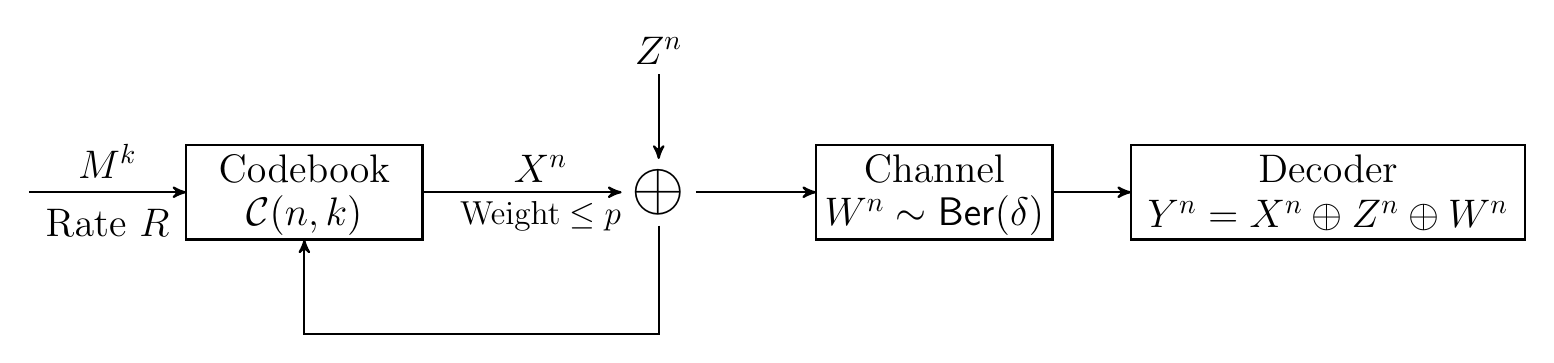
\begin{tikzpicture}
  [yscale=0.8,node distance=1cm,draw=black,thick, >=stealth']

  \def \reclen {3}
  \def \linelen {2}
  \def \recwid {0.75}

  \draw[->] (-1,0) -- (-1+\linelen,0);
  \draw (0+\linelen-1,\recwid) rectangle (0+\linelen+\reclen-1,-\recwid);
  \node (sideinfnode) at (0+\linelen+\reclen+\linelen,0) {\Huge{$\oplus$}};
  \draw[->] (0+\linelen+\reclen-1,0) -- (sideinfnode);
  \draw[->] (sideinfnode) -- (0+\linelen+\reclen+\linelen+\linelen,0);
  \node (znlabel) at (0+\linelen+\reclen+\linelen,3*\recwid) {\Large{$Z^n$}};
  \draw[->] (znlabel) -- (sideinfnode);
  \draw[->] (sideinfnode) -- (0+\linelen+\reclen+\linelen,-3*\recwid) -- (\linelen+0.5*\reclen-1,-3*\recwid) -- (\linelen+0.5*\reclen-1,-\recwid);
  \draw (0+\linelen+\reclen+\linelen+\linelen,\recwid) rectangle (0+\linelen+\reclen+\linelen+\linelen+\reclen,-\recwid);
  \draw[->] (0+\linelen+\reclen+\linelen+\linelen+\reclen,0) -- (0+\linelen+\reclen+\linelen+\linelen+\reclen+0.5*\linelen,0);
  \draw (0+\linelen+\reclen+\linelen+\reclen+\linelen+0.5*\linelen,\recwid) rectangle (0+\linelen+\reclen+\linelen+\reclen+\linelen+\reclen+1.5*\linelen,-\recwid);

  \node at (\linelen+0.5*\reclen-1,0.5*\recwid) {\Large{Codebook}};
  \node at (\linelen+0.5*\reclen-1,-0.5*\recwid) {\Large{$\mathcal{C}(n,k)$}};

  \node at (3*\linelen+1.5*\reclen,0.5*\recwid) {\Large{Channel}};
  \node at (3*\linelen+1.5*\reclen,-0.5*\recwid) {\Large{$W^n \sim \mathsf{Ber}(\delta)$}};

  \node at (4*\linelen+2.5*\reclen,0.5*\recwid) {\Large{Decoder}};
  \node at (4*\linelen+2.5*\reclen,-0.5*\recwid) {\Large{$Y^n=X^n\oplus Z^n \oplus W^n$}};

  \node at (0.5*\linelen-1,0.65*\recwid) {\Large{$M^k$}};
  \node at (0.5*\linelen-1,-0.65*\recwid) {\Large{Rate $R$}};
  \node at (1.5*\linelen+\reclen-0.5,0.5*\recwid) {\Large{$X^n$}};
  \node at (1.5*\linelen+\reclen-0.5,-0.5*\recwid) {\large{$\mathrm{Weight}\leq p$}};

\end{tikzpicture}

%%% Local Variables: 
%%% mode: latex
%%% TeX-master: "../talk"
%%% End: 
}
  \end{center}
  \begin{block}{Gelfand-Pinsker Formulation}<2->
    \begin{itemize}
    \item<2-> Message $M^k$ encoded to $X^n \in \mathcal{C}$ with \textcolor{blue}{$\tfrac{1}{n} \sum_{i=1}^n \expt[X_i] \leq p \leq \frac{1}{2}$}
    \item<2-> Side-information $Z^n$ is available \alert{only at the encoder}
    \item<3-> The output at the decoder is
      \begin{align*}
        Y^n=X^n\oplus Z^n \oplus W^n, \quad \{W_i\} \sim \textsf{Ber}(\delta)
      \end{align*}
    \item<4-> Capacity region by Gelfand-Pinsker:
      \begin{align*}
        R < h(p) - h(\delta)
      \end{align*}
    \end{itemize}
  \end{block}
\end{frame}

\begin{frame}{Main Result}
  \begin{block}{Objective}<1->
    \begin{itemize}
    \item Construct \alert{low-complexity} coding schemes that achieve the \textcolor{blue}{complete rate regions} of Wyner-Ziv and Gelfand-Pinsker \vspace{0.1cm}
      \begin{itemize}
      \item Low-complexity encoding and decoding
      \end{itemize}
    \end{itemize}
  \end{block}
  \vspace{0.1cm}
  \begin{block}{Idea}<2->
    \begin{itemize}
    \item Wainwright et al.~used compound LDGM/LDPC codes with \alert{optimal encoding/decoding}\vspace{0.1cm}
    \item Message-passing algorithms have \textcolor{blue}{non-negligible gap}\vspace{0.1cm}
    \item<3-> Remedy via \alert{Spatial-Coupling}
      \begin{itemize}
      \item Channel coding in coupled compound codes (Kasai et al.)
      \item Lossy source coding with spatially-coupled LDGM (Aref et al.)
      \item Encoding with \alert{compound codes has additional challenges}
      \end{itemize}
    \end{itemize}
  \end{block}
\end{frame}

% \begin{frame}{A Brief History}
%   \begin{itemize}
%   \item Item 1
%   \item Item 2
%   \end{itemize}
% \end{frame}

\begin{frame}{Compound LDGM/LDPC Codes}
  \begin{columns}
    \column{0.45\textwidth}
    \begin{center}
      \setlength\tikzheight{5cm}
      \setlength\tikzwidth{6cm}
      \scalebox{0.5}{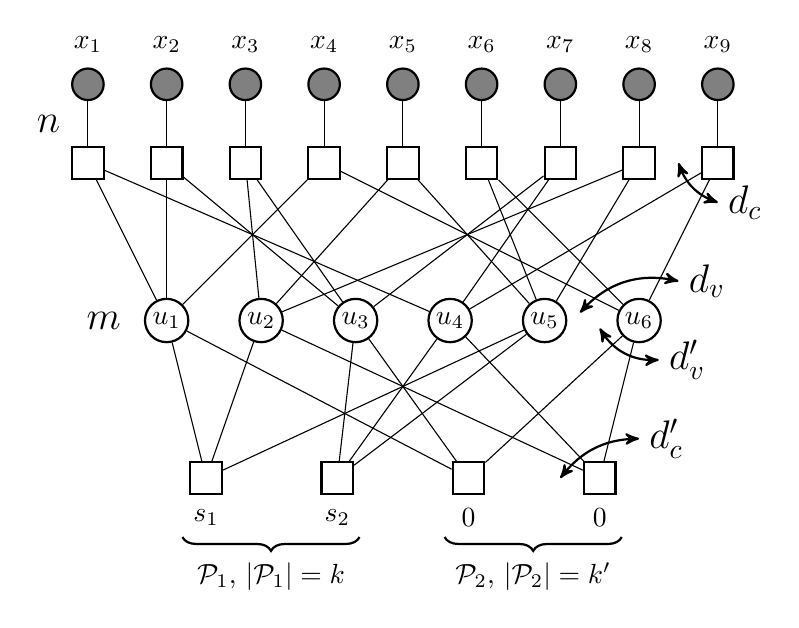
\begin{tikzpicture}
  [
  node distance = 12mm, draw=black, thick, >=stealth',
  bitnode/.style={circle, inner sep = 0pt, minimum size = 5.5mm, draw=black},
  checknode/.style={rectangle, inner sep = 0pt, minimum size = 4mm, draw=black},
  bitnode2/.style={circle, inner sep = 0pt, minimum size = 4mm, draw=black, fill=black!50},
  ]
  
  \foreach \x in {1,2,...,9} {
    \node[bitnode2] (bb\x) at (\x-5,3) {};
  }

  \foreach \y in {1,2,...,9} {
    \node at (\y-5,3.5) {$x_{\y}$};
  }

  \foreach \x in {1,2,...,9} {
    \node[checknode] (c\x) at (\x-5,2) {};
    \draw[thin] (c\x) -- (bb\x);
  }

  \foreach \x in {1,2,...,6} {
    \node[bitnode] (b\x) at (1.2*\x-4.2,0) {$u_{\x}$};
  }

  \foreach \x in {1,...,4} {
    \node[checknode] (cc\x) at (5*\x/3-2.5-5/3,-2) {};
  }

  \draw[thin] (c1) -- (b4);
  \draw[thin] (c1) -- (b1);
  \draw[thin] (c2) -- (b1);
  \draw[thin] (c2) -- (b3);
  \draw[thin] (c3) -- (b3);
  \draw[thin] (c3) -- (b2);
  \draw[thin] (c4) -- (b1);
  \draw[thin] (c4) -- (b6);
  \draw[thin] (c5) -- (b2);
  \draw[thin] (c5) -- (b5);
  \draw[thin] (c6) -- (b5);
  \draw[thin] (c6) -- (b6);
  \draw[thin] (c7) -- (b3);
  \draw[thin] (c7) -- (b4);
  \draw[thin] (c8) -- (b5);
  \draw[thin] (c8) -- (b2);
  \draw[thin] (c9) -- (b4);
  \draw[thin] (c9) -- (b6);


  \draw[thin] (cc1) -- (b2);
  \draw[thin] (cc1) -- (b1);
  \draw[thin] (cc1) -- (b5);
  \draw[thin] (cc2) -- (b5);
  \draw[thin] (cc2) -- (b3);
  \draw[thin] (cc2) -- (b4);
  \draw[thin] (cc3) -- (b1);
  \draw[thin] (cc3) -- (b3);
  \draw[thin] (cc3) -- (b6);
  \draw[thin] (cc4) -- (b2);
  \draw[thin] (cc4) -- (b6);
  \draw[thin] (cc4) -- (b4);

  \draw[<->] (3.5,2) to [bend right=25] (4,1.5) node [right] {\Large $d_{c}$};
  \draw[<->] (2.25,0.1) to [bend left=30] (3.5,0.5) node [right] {\Large $d_{v}$};
  \draw[<->] (2.5,-0.1) to [bend right=30] (3.25,-0.5) node [right] {\Large $d'_{v}$};
  \draw[<->] (2,-2) to [bend left=25] (3,-1.5) node [right] {\Large $d'_{c}$};

  \node at (-4.5,2.5) {\Large $n$};
  \node at (-3.8,0) {\Large $m$};

  \node at (5*1/3-2.5-5/3,-2.5) {$s_1$};
  \node at (5*2/3-2.5-5/3,-2.5) {$s_2$};
  \node at (5*3/3-2.5-5/3,-2.5) {$0$};
  \node at (5*4/3-2.5-5/3,-2.5) {$0$};

  \draw[decorate,decoration={brace,amplitude=5pt,mirror}] (-2.8,-2.75) -- (-0.55,-2.75) node [midway,yshift=-0.5cm] {$\mathcal{P}_1$,  $|\mathcal{P}_1|=k$};
  \draw[decorate,decoration={brace,amplitude=5pt,mirror}] (3.33-2.8,-2.75) -- (3.33-0.55,-2.75) node [midway,yshift=-0.5cm]{$\mathcal{P}_2$,  $|\mathcal{P}_2|=k'$};
\end{tikzpicture}

%%% Local Variables: 
%%% mode: latex
%%% TeX-master: "../isit14"
%%% End: 
}
    \end{center}
    \column{0.55\textwidth}
    \begin{itemize}
    \item Codebook $\mathcal{C}(n,m-k-k')$ \vspace{0.1cm}
    \item \textcolor{blue}{Message constraints} \vspace{-0.2cm}
      \begin{align*}
        u_1\oplus u_2 \oplus u_5&=s_1, &  u_1\oplus u_3 \oplus u_6&=0
      \end{align*}
    \item Codeword $(x_1,\cdots,x_9)$: \vspace{-0.2cm}
      \begin{align*}
        x_1 &= u_1 \oplus u_4, & x_2 &= \cdots
      \end{align*}
    \end{itemize}
  \end{columns}
  \vspace{0.2cm}
  \begin{block}{Key Properties}<2->
    \begin{itemize}
    \item Compound code is 
      \begin{itemize}
      \item a \alert{good source code} under optimal encoding
      \item a \alert{good channel code} under optimal decoding
      \end{itemize}
    % \item LDGM code is 
    %   \begin{itemize}
    %   \item a \alert{good source code} under optimal encoding
    %   \item \textcolor{blue}{(side note)} LDGM code is \alert{not} a good channel code
    %   \end{itemize}
    \end{itemize}
  \end{block}
\end{frame}

\begin{frame}{Good Code}
  \begin{block}{``Good'' source code}
    \begin{itemize}
    \item Rate of the code is $R=1-h(D)+\varepsilon$
    \item When this code is used to \alert{optimally encode} $\mathsf{Ber}(\tfrac{1}{2})$
    \item The average Hamming \textcolor{blue}{distortion is at most $D$}
    \end{itemize}
  \end{block}
  \vspace{0.4cm}
  \begin{block}{``Good'' channel code}
    \begin{itemize}
    \item Rate of the code is $R=1-h(\delta)-\varepsilon$
    \item When this code is used for channel coding on $\mathsf{BSC}(\delta)$
    \item Message est.~under \alert{optimal decoding} with \textcolor{blue}{error at most $\varepsilon$}
    \end{itemize}
  \end{block}
\end{frame}

% \begin{frame}{Coding Scheme: Wyner-Ziv}
%   \vspace{-0.2cm}
%   \begin{center}
%     \scalebox{0.5}{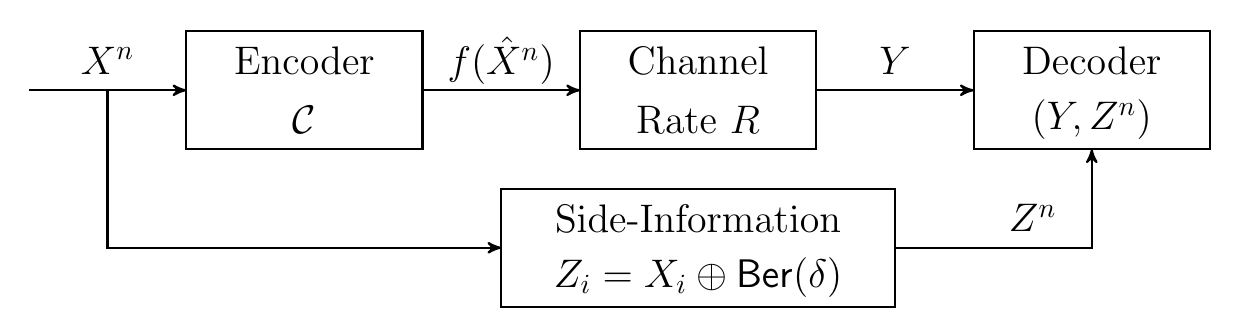
\begin{tikzpicture}
  [node distance=1cm,draw=black,thick, >=stealth']

  \def \reclen {3}
  \def \linelen {2}
  \def \recwid {0.75}

  \draw[->] (0,0) -- (0+\linelen,0);
  \draw (0+\linelen,\recwid) rectangle (0+\linelen+\reclen,-\recwid);
  \draw[->] (0+\linelen+\reclen,0) -- (0+\linelen+\reclen+\linelen,0);
  \draw (0+\linelen+\reclen+\linelen,\recwid) rectangle (0+\linelen+\reclen+\linelen+\reclen,-\recwid);
  \draw[->] (0+\linelen+\reclen+\linelen+\reclen,0) -- (0+\linelen+\reclen+\linelen+\reclen+\linelen,0);
  \draw (0+\linelen+\reclen+\linelen+\reclen+\linelen,\recwid) rectangle (0+\linelen+\reclen+\linelen+\reclen+\linelen+\reclen,-\recwid);

  \draw[->] (0.5*\linelen,0) -- (0.5*\linelen,-2) -- (1.5*\linelen+\reclen,-2);
  \draw (1.5*\linelen+\reclen,-2+\recwid) rectangle (2.5*\linelen+2*\reclen,-2-\recwid);
  \draw[->] (2.5*\linelen+2*\reclen,-2) -- (2*\linelen+2*\reclen+\linelen+0.5*\reclen,-2) -- (2*\linelen+2*\reclen+\linelen+0.5*\reclen,-\recwid);

  \node at (\linelen+0.5*\reclen,0.5*\recwid) {\Large{Encoder}};
  \node at (\linelen+0.5*\reclen,-0.5*\recwid) {\Large{$\mathcal{C}$}};

  \node at (2*\linelen+1.5*\reclen,0.5*\recwid) {\Large{Channel}};
  \node at (2*\linelen+1.5*\reclen,-0.5*\recwid) {\Large{Rate $R$}};

  \node at (3*\linelen+2.5*\reclen,0.5*\recwid) {\Large{Decoder}};
  \node at (3*\linelen+2.5*\reclen,-0.5*\recwid) {\Large{$(Y,Z^n)$}};

  \node at (2*\linelen+1.5*\reclen,-2+0.5*\recwid) {\Large{Side-Information}};
  \node at (2*\linelen+1.5*\reclen,-2-0.5*\recwid) {\Large{$Z_i=X_i\oplus \mathsf{Ber}(\delta)$}};

  \node at (0.5*\linelen,0.5*\recwid) {\Large{$X^n$}};
  \node at (1.5*\linelen+\reclen,0.5*\recwid) {\Large{$f(\hat{X}^n)$}};
  \node at (2.5*\linelen+2*\reclen,0.5*\recwid) {\Large{$Y$}};
  \node at (3*\linelen+2.25*\reclen,-2+0.5*\recwid) {\Large{$Z^n$}};

\end{tikzpicture}

%%% Local Variables: 
%%% mode: latex
%%% TeX-master: "../talk"
%%% End: 
}
%   \end{center}
%   \vspace{-0.35cm}
%   \begin{columns}
%     \column{0.5\textwidth}
%     \vspace{-0.5cm}
%     \begin{center}
%       \setlength\tikzheight{5cm}
%       \setlength\tikzwidth{6cm}
%       \scalebox{0.5}{\begin{tikzpicture}
  [
  node distance = 12mm, draw=black, thick, >=stealth',
  bitnode/.style={circle, inner sep = 0pt, minimum size = 5.5mm, draw=black},
  bitnodehidden/.style={circle, inner sep = 0pt, minimum size = 5.5mm, draw=white},
  checknode/.style={rectangle, inner sep = 0pt, minimum size = 4mm, draw=black},
  checknodehidden/.style={rectangle, inner sep = 0pt, minimum size = 4mm, draw=white},
  bitnode2/.style={circle, inner sep = 0pt, minimum size = 4mm, draw=black, fill=black!50},
  bitnode2hidden/.style={circle, inner sep = 0pt, minimum size = 4mm, draw=white, fill=white},
  ]

  \only<1>{

    \foreach \x in {1,2,...,9} {
      \node[bitnode2hidden] (bb\x) at (\x-5,3) {};
    }

    \foreach \y in {1,2,...,9} {
      \node[white] at (\y-5,4.5) {\Large{$x_{\y}$}};
    }

    \foreach \y in {1,2,...,9} {
      \node[white] at (\y-5,3.5) {\Large{$\hat{x}_{\y}$}};
    }

    \foreach \x in {1,2,...,9} {
      \node[checknodehidden] (c\x) at (\x-5,2) {};
      \draw[white,thin] (c\x) -- (bb\x);
    }

    \foreach \x in {1,2,...,6} {
      \node[bitnodehidden,white] (b\x) at (1.2*\x-4.2,0) {$u_{\x}$};
    }

    \node[white] at (-4.5,2.5) {\Large $n$};
    \node[white] at (-3.8,0) {\Large $m$};

    \draw[white,thin] (c1) -- (b4);
    \draw[white,thin] (c1) -- (b1);
    \draw[white,thin] (c2) -- (b1);
    \draw[white,thin] (c2) -- (b3);
    \draw[white,thin] (c3) -- (b3);
    \draw[white,thin] (c3) -- (b2);
    \draw[white,thin] (c4) -- (b1);
    \draw[white,thin] (c4) -- (b6);
    \draw[white,thin] (c5) -- (b2);
    \draw[white,thin] (c5) -- (b5);
    \draw[white,thin] (c6) -- (b5);
    \draw[white,thin] (c6) -- (b6);
    \draw[white,thin] (c7) -- (b3);
    \draw[white,thin] (c7) -- (b4);
    \draw[white,thin] (c8) -- (b5);
    \draw[white,thin] (c8) -- (b2);
    \draw[white,thin] (c9) -- (b4);
    \draw[white,thin] (c9) -- (b6);

    \foreach \x in {1,...,4} {
      \node[checknodehidden] (cc\x) at (5*\x/3-2.5-5/3,-2) {};
    }
    \node[white] at (-3.8,-2) {\Large $k$};

    \draw[white,thin] (cc1) -- (b2);
    \draw[white,thin] (cc1) -- (b1);
    \draw[white,thin] (cc1) -- (b5);
    \draw[white,thin] (cc2) -- (b5);
    \draw[white,thin] (cc2) -- (b3);
    \draw[white,thin] (cc2) -- (b4);
    \draw[white,thin] (cc3) -- (b1);
    \draw[white,thin] (cc3) -- (b3);
    \draw[white,thin] (cc3) -- (b6);
    \draw[white,thin] (cc4) -- (b2);
    \draw[white,thin] (cc4) -- (b6);
    \draw[white,thin] (cc4) -- (b4);

    \node[white] at (5*1/3-2.5-5/3,-2.5) {$s_1$};
    \node[white] at (5*2/3-2.5-5/3,-2.5) {$s_2$};
    \node[white] at (5*3/3-2.5-5/3,-2.5) {$s_3$};
    \node[white] at (5*4/3-2.5-5/3,-2.5) {$s_4$};

    \draw[white,decorate,decoration={brace,amplitude=5pt,mirror}] (-2.8,-2.75) -- (3.33-0.55,-2.75) node [midway,yshift=-0.5cm] {$\mathcal{P}_1$,  $|\mathcal{P}_1|=k$};

    \node[white] at (-3,-4.25) {\LARGE{$\frac{m}{n}\approx 1 - h(D) + \varepsilon$}};
    \node[white] at (3,-4.25) {\LARGE{$\frac{m-k}{n}\approx 1 - h(D*\delta) + \varepsilon$}};
  }

  \only<2->{
    \foreach \x in {1,2,...,9} {
      \node[bitnode2] (bb\x) at (\x-5,3) {};
    }

    \foreach \y in {1,2,...,9} {
      \node at (\y-5,4.5) {\Large{$x_{\y}$}};
    }

    \foreach \y in {1,2,...,9} {
      \node at (\y-5,3.5) {\Large{$\hat{x}_{\y}$}};
    }

    \foreach \x in {1,2,...,9} {
      \node[checknode] (c\x) at (\x-5,2) {};
      \draw[thin] (c\x) -- (bb\x);
    }

    \foreach \x in {1,2,...,6} {
      \node[bitnode] (b\x) at (1.2*\x-4.2,0) {$u_{\x}$};
    }

    \node at (-4.5,2.5) {\Large $n$};
    \node at (-3.8,0) {\Large $m$};

    \draw[thin] (c1) -- (b4);
    \draw[thin] (c1) -- (b1);
    \draw[thin] (c2) -- (b1);
    \draw[thin] (c2) -- (b3);
    \draw[thin] (c3) -- (b3);
    \draw[thin] (c3) -- (b2);
    \draw[thin] (c4) -- (b1);
    \draw[thin] (c4) -- (b6);
    \draw[thin] (c5) -- (b2);
    \draw[thin] (c5) -- (b5);
    \draw[thin] (c6) -- (b5);
    \draw[thin] (c6) -- (b6);
    \draw[thin] (c7) -- (b3);
    \draw[thin] (c7) -- (b4);
    \draw[thin] (c8) -- (b5);
    \draw[thin] (c8) -- (b2);
    \draw[thin] (c9) -- (b4);
    \draw[thin] (c9) -- (b6);
  }



  \only<2>{
    \foreach \x in {1,...,4} {
      \node[checknodehidden] (cc\x) at (5*\x/3-2.5-5/3,-2) {};
    }

    \draw[white,thin] (cc1) -- (b2);
    \draw[white,thin] (cc1) -- (b1);
    \draw[white,thin] (cc1) -- (b5);
    \draw[white,thin] (cc2) -- (b5);
    \draw[white,thin] (cc2) -- (b3);
    \draw[white,thin] (cc2) -- (b4);
    \draw[white,thin] (cc3) -- (b1);
    \draw[white,thin] (cc3) -- (b3);
    \draw[white,thin] (cc3) -- (b6);
    \draw[white,thin] (cc4) -- (b2);
    \draw[white,thin] (cc4) -- (b6);
    \draw[white,thin] (cc4) -- (b4);

    \node[white] at (-3.8,-2) {\Large $k$};

    \node[white] at (5*1/3-2.5-5/3,-2.5) {$s_1$};
    \node[white] at (5*2/3-2.5-5/3,-2.5) {$s_2$};
    \node[white] at (5*3/3-2.5-5/3,-2.5) {$s_3$};
    \node[white] at (5*4/3-2.5-5/3,-2.5) {$s_4$};

    \draw[white,decorate,decoration={brace,amplitude=5pt,mirror}] (-2.8,-2.75) -- (3.33-0.55,-2.75) node [midway,yshift=-0.5cm] {$\mathcal{P}_1$,  $|\mathcal{P}_1|=k$};

    \node at (-3,-4.25) {\LARGE{$\frac{m}{n}\approx 1 - h(D) + \varepsilon$}};
    \node[white] at (3,-4.25) {\LARGE{$\frac{m-k}{n}\approx 1 - h(D*\delta) + \varepsilon$}};
  }

  \only<3->{
    \foreach \x in {1,...,4} {
      \node[checknode] (cc\x) at (5*\x/3-2.5-5/3,-2) {};
    }
    \node at (-3.8,-2) {\Large $k$};

    \draw[thin] (cc1) -- (b2);
    \draw[thin] (cc1) -- (b1);
    \draw[thin] (cc1) -- (b5);
    \draw[thin] (cc2) -- (b5);
    \draw[thin] (cc2) -- (b3);
    \draw[thin] (cc2) -- (b4);
    \draw[thin] (cc3) -- (b1);
    \draw[thin] (cc3) -- (b3);
    \draw[thin] (cc3) -- (b6);
    \draw[thin] (cc4) -- (b2);
    \draw[thin] (cc4) -- (b6);
    \draw[thin] (cc4) -- (b4);


    \node at (5*1/3-2.5-5/3,-2.5) {$s_1$};
    \node at (5*2/3-2.5-5/3,-2.5) {$s_2$};
    \node at (5*3/3-2.5-5/3,-2.5) {$s_3$};
    \node at (5*4/3-2.5-5/3,-2.5) {$s_4$};

    \draw[decorate,decoration={brace,amplitude=5pt,mirror}] (-2.8,-2.75) -- (3.33-0.55,-2.75) node [midway,yshift=-0.5cm] {$\mathcal{P}_1$,  $|\mathcal{P}_1|=k$};

    \node at (-3,-4.25) {\LARGE{$\frac{m}{n}\approx 1 - h(D) + \varepsilon$}};
    \node at (3,-4.25) {\LARGE{$\frac{m-k}{n}\approx 1 - h(D*\delta) + \varepsilon$}};
  }

\end{tikzpicture}


%%% Local Variables: 
%%% mode: latex
%%% TeX-master: "../talk"
%%% End: 
}
%     \end{center}
%     \column{0.5\textwidth}
%     \begin{itemize}
%     \item<2-> Encode $X^n$ to $\hat{X}^n$ using \alert{LDGM} w/ Distortion $\approx D$ \vspace{0.1cm}
%     \item<3-> Compute \& \textcolor{blue}{transmit $s_i$'s} \vspace{0.1cm} \small{$R = \frac{k}{n} \approx h(D*\delta) - h(D)$} \vspace{0.1cm}
%     \item <3-> Decoder has $Z^n$: \vspace{-0.2cm}
%       \small{
%         \begin{align*}
%           Z_i &= X_i \oplus \mathsf{Ber}(\delta) \\
%           &\approx \hat{X_i} \oplus \mathsf{Ber}(D) \oplus \mathsf{Ber}(\delta) \\
%           &= \hat{X_i} \oplus \mathsf{Ber}(D*\delta)
%         \end{align*}
%       }
%     \item <3-> Decode $\hat{X}^n$ from $Z^n$ \& $s_i$
%     \end{itemize}
%   \end{columns}
% \end{frame}

\begin{frame}{Coding Scheme: Gelfand-Pinsker}
  \begin{center}
    \scalebox{0.5}{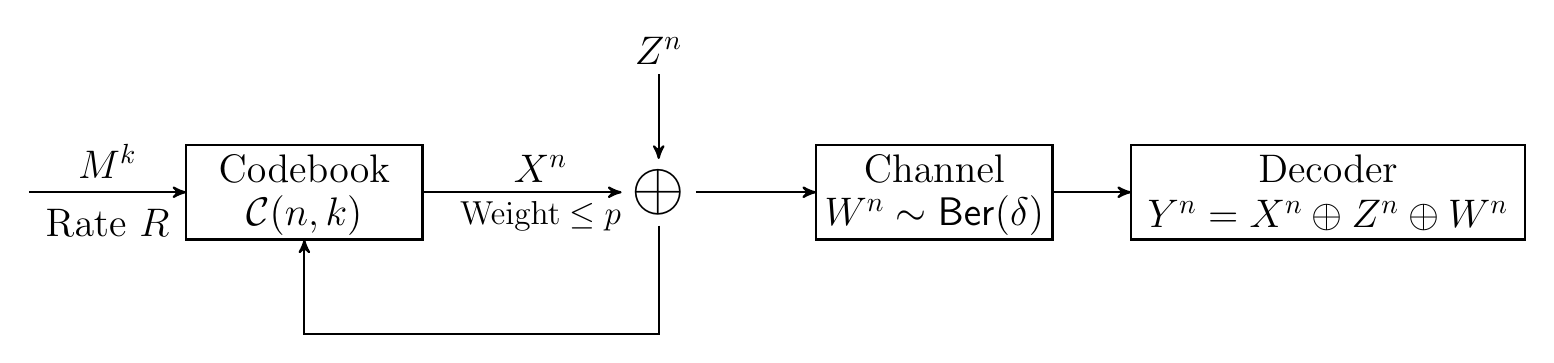
\begin{tikzpicture}
  [yscale=0.8,node distance=1cm,draw=black,thick, >=stealth']

  \def \reclen {3}
  \def \linelen {2}
  \def \recwid {0.75}

  \draw[->] (-1,0) -- (-1+\linelen,0);
  \draw (0+\linelen-1,\recwid) rectangle (0+\linelen+\reclen-1,-\recwid);
  \node (sideinfnode) at (0+\linelen+\reclen+\linelen,0) {\Huge{$\oplus$}};
  \draw[->] (0+\linelen+\reclen-1,0) -- (sideinfnode);
  \draw[->] (sideinfnode) -- (0+\linelen+\reclen+\linelen+\linelen,0);
  \node (znlabel) at (0+\linelen+\reclen+\linelen,3*\recwid) {\Large{$Z^n$}};
  \draw[->] (znlabel) -- (sideinfnode);
  \draw[->] (sideinfnode) -- (0+\linelen+\reclen+\linelen,-3*\recwid) -- (\linelen+0.5*\reclen-1,-3*\recwid) -- (\linelen+0.5*\reclen-1,-\recwid);
  \draw (0+\linelen+\reclen+\linelen+\linelen,\recwid) rectangle (0+\linelen+\reclen+\linelen+\linelen+\reclen,-\recwid);
  \draw[->] (0+\linelen+\reclen+\linelen+\linelen+\reclen,0) -- (0+\linelen+\reclen+\linelen+\linelen+\reclen+0.5*\linelen,0);
  \draw (0+\linelen+\reclen+\linelen+\reclen+\linelen+0.5*\linelen,\recwid) rectangle (0+\linelen+\reclen+\linelen+\reclen+\linelen+\reclen+1.5*\linelen,-\recwid);

  \node at (\linelen+0.5*\reclen-1,0.5*\recwid) {\Large{Codebook}};
  \node at (\linelen+0.5*\reclen-1,-0.5*\recwid) {\Large{$\mathcal{C}(n,k)$}};

  \node at (3*\linelen+1.5*\reclen,0.5*\recwid) {\Large{Channel}};
  \node at (3*\linelen+1.5*\reclen,-0.5*\recwid) {\Large{$W^n \sim \mathsf{Ber}(\delta)$}};

  \node at (4*\linelen+2.5*\reclen,0.5*\recwid) {\Large{Decoder}};
  \node at (4*\linelen+2.5*\reclen,-0.5*\recwid) {\Large{$Y^n=X^n\oplus Z^n \oplus W^n$}};

  \node at (0.5*\linelen-1,0.65*\recwid) {\Large{$M^k$}};
  \node at (0.5*\linelen-1,-0.65*\recwid) {\Large{Rate $R$}};
  \node at (1.5*\linelen+\reclen-0.5,0.5*\recwid) {\Large{$X^n$}};
  \node at (1.5*\linelen+\reclen-0.5,-0.5*\recwid) {\large{$\mathrm{Weight}\leq p$}};

\end{tikzpicture}

%%% Local Variables: 
%%% mode: latex
%%% TeX-master: "../talk"
%%% End: 
}
  \end{center}
  \vspace{-0.4cm}
  \begin{columns}
    \column{0.5\textwidth}
    \begin{center}
      \setlength\tikzheight{5cm}
      \setlength\tikzwidth{6cm}
      \scalebox{0.5}{\input{Figures/gelfand-pinsker-coding}}
    \end{center}
    \column{0.5\textwidth}
    \begin{itemize}
    \item<2-> With message $M^k$, encode $Z^n$ to $\hat{Z}^n$ (Distortion $\approx p$) \vspace{0.1cm}
    \item<2-> \textcolor{red}{Transmit $X^n=Z^n \oplus \hat{Z}^n$} \vspace{0.1cm}
    \item<3-> Decoder has \vspace{-0.2cm}
      \small{
        \begin{align*}
          Y^n&=X^n \oplus Z^n \oplus W^n\\
          &= \hat{Z}^n \oplus W^n 
        \end{align*}
      }
    \item <3-> \textcolor{blue}{Decode $\hat{Z}^n$ and compute $M^k$}
    \item <4-> $R=\tfrac{k}{n}\approx h(p)-h(\delta)$
    \end{itemize}
  \end{columns}
\end{frame}

\begin{frame}{Remarks}
  \begin{itemize}
  \item Need codes that are \alert{simultaneously good} for channel and source coding \vspace{0.2cm}
  \item Use \textcolor{blue}{message-passing algorithms} instead of \alert{optimal} \vspace{0.2cm}
  \item Use spatial-coupling for \alert{goodness} of codes under message-passing \vspace{0.2cm}
  \end{itemize}
\end{frame}

\begin{frame}{Spatially-Coupled Compound LDGM/LDPC Codes}
  \begin{center}
    \scalebox{0.8}{\begin{tikzpicture}[
  xscale=0.33,yscale=1,
  bitnode/.style={circle,minimum size=10pt,thick,draw=black,fill=white},
  bitnodeblack/.style={circle,minimum size=10pt,thick,draw=black,fill=white},
  bitnodewhite/.style={circle,minimum size=10pt,thick,draw=white,fill=white},
  bitnode2/.style={circle,minimum size=10pt,thick,draw=black,fill=gray},
  bitnode2black/.style={circle,minimum size=10pt,thick,draw=black,fill=gray},
  bitnode2white/.style={circle,minimum size=10pt,thick,draw=white,fill=white},
  checknode/.style={rectangle,minimum size=8pt,thick,draw=black,fill=white},
  checknodeblack/.style={rectangle,minimum size=8pt,thick,draw=black,fill=white},
  checknodewhite/.style={rectangle,minimum size=8pt,thick,draw=white,fill=white},
  permnode/.style={rectangle,very thin,minimum width=30pt,minimum height=18pt,fill=white,draw=black},
  permnodeblack/.style={rectangle,very thin,minimum width=30pt,minimum height=18pt,fill=white,draw=black},
  permnodewhite/.style={rectangle,very thin,minimum width=30pt,minimum height=18pt,fill=white,draw=white},
  permedge/.style={black!65},
  permedgeblack/.style={black!65},
  permedgewhite/.style={white},
  ]

  \def \cndist {0.75}
  \def \vndist {0.75}
  \def \ccndist {0.75}
  \def \vvny {2.75}
  \def \cny {2}
  \def \vny {-2}
  \def \ccny {-6}

  \def \midx   {0.5}

  \only<1>{
    \foreach \x/\i/\col in {0/1/white,6/2/white,12/3/white,18/4/black,24/5/white,30/6/white,36/7/white} {
      \draw[\col] (\x-\cndist, \cny) +(0,0) -- +(240:1);
      \draw[\col] (\x-\cndist, \cny) +(0,0) -- +(255:1);
      \draw[\col] (\x-\cndist, \cny) +(0,0) -- +(270:1);
      \draw[\col] (\x-\cndist, \cny) +(0,0) -- +(285:1);
      \draw[\col] (\x-\cndist, \cny) +(0,0) -- +(300:1);

      \draw[\col] (\x+\cndist, \cny) +(0,0) -- +(240:1);
      \draw[\col] (\x+\cndist, \cny) +(0,0) -- +(255:1);
      \draw[\col] (\x+\cndist, \cny) +(0,0) -- +(270:1);
      \draw[\col] (\x+\cndist, \cny) +(0,0) -- +(285:1);
      \draw[\col] (\x+\cndist, \cny) +(0,0) -- +(300:1);

      \draw[\col] (\x-\vndist, \vny) +(0,0) -- +(52.5:1);
      \draw[\col] (\x-\vndist, \vny) +(0,0) -- +(67.5:1);
      \draw[\col] (\x-\vndist, \vny) +(0,0) -- +(82.5:1);
      \draw[\col] (\x-\vndist, \vny) +(0,0) -- +(97.5:1);
      \draw[\col] (\x-\vndist, \vny) +(0,0) -- +(112.5:1);
      \draw[\col] (\x-\vndist, \vny) +(0,0) -- +(127.5:1);

      \draw[\col] (\x+\vndist, \vny) +(0,0) -- +(52.5:1);
      \draw[\col] (\x+\vndist, \vny) +(0,0) -- +(67.5:1);
      \draw[\col] (\x+\vndist, \vny) +(0,0) -- +(82.5:1);
      \draw[\col] (\x+\vndist, \vny) +(0,0) -- +(97.5:1);
      \draw[\col] (\x+\vndist, \vny) +(0,0) -- +(112.5:1);
      \draw[\col] (\x+\vndist, \vny) +(0,0) -- +(127.5:1);

      \draw[\col] (\x-\vndist, \vny) +(0,0) -- +(240:1);
      \draw[\col] (\x-\vndist, \vny) +(0,0) -- +(255:1);
      \draw[\col] (\x-\vndist, \vny) +(0,0) -- +(270:1);
      \draw[\col] (\x-\vndist, \vny) +(0,0) -- +(285:1);
      \draw[\col] (\x-\vndist, \vny) +(0,0) -- +(300:1);

      \draw[\col] (\x+\vndist, \vny) +(0,0) -- +(240:1);
      \draw[\col] (\x+\vndist, \vny) +(0,0) -- +(255:1);
      \draw[\col] (\x+\vndist, \vny) +(0,0) -- +(270:1);
      \draw[\col] (\x+\vndist, \vny) +(0,0) -- +(285:1);
      \draw[\col] (\x+\vndist, \vny) +(0,0) -- +(300:1);

      \draw[\col] (\x-\vndist, \ccny) +(0,0) -- +(52.5:1);
      \draw[\col] (\x-\vndist, \ccny) +(0,0) -- +(67.5:1);
      \draw[\col] (\x-\vndist, \ccny) +(0,0) -- +(82.5:1);
      \draw[\col] (\x-\vndist, \ccny) +(0,0) -- +(97.5:1);
      \draw[\col] (\x-\vndist, \ccny) +(0,0) -- +(112.5:1);
      \draw[\col] (\x-\vndist, \ccny) +(0,0) -- +(127.5:1);

      \draw[\col] (\x+\vndist, \ccny) +(0,0) -- +(52.5:1);
      \draw[\col] (\x+\vndist, \ccny) +(0,0) -- +(67.5:1);
      \draw[\col] (\x+\vndist, \ccny) +(0,0) -- +(82.5:1);
      \draw[\col] (\x+\vndist, \ccny) +(0,0) -- +(97.5:1);
      \draw[\col] (\x+\vndist, \ccny) +(0,0) -- +(112.5:1);
      \draw[\col] (\x+\vndist, \ccny) +(0,0) -- +(127.5:1);

      \node[checknode\col] (c1\i) at (\x-\cndist, \cny) {};
      \node[checknode\col] (c2\i) at (\x+\cndist, \cny) {};
      \node[bitnode\col] (v1\i) at (\x-\vndist, \vny) {};
      \node[bitnode\col] (v2\i) at (\x+\vndist, \vny) {};
      \node[checknode\col] (cc1\i) at (\x-\ccndist, \ccny) {};
      \node[checknode\col] (cc2\i) at (\x+\ccndist, \ccny) {};

      \node[bitnode2\col] (vv1\i) at (\x-\cndist,\vvny) {};
      \node[bitnode2\col] (vv2\i) at (\x+\cndist,\vvny) {};
      \draw[\col] (vv1\i) -- (c1\i);
      \draw[\col] (vv2\i) -- (c2\i);

      \foreach \j in {-5.7,-2.3,-1.7,1.7} {
        \node[\col] at (\x,\j) {\tiny{$...$}};
      }

      \node[permnode\col] (perm1_node\i) at (\x,\cny-1) {\textcolor{\col}{\footnotesize{$\pi$}}};
      \node[permnode\col] (perm2_node\i) at (\x,\vny+1) {\textcolor{\col}{\footnotesize{$\pi$}}};   
      \node[permnode\col] (perm3_node\i) at (\x,\vny-1) {\textcolor{\col}{\footnotesize{$\pi$}}};
      \node[permnode\col] (perm4_node\i) at (\x,\ccny+1) {\textcolor{\col}{\footnotesize{$\pi$}}};

      \draw[permedge\col] (perm1_node\i) .. controls (\x-0.2,0) .. (perm2_node\i);
      \draw[permedge\col] (perm1_node\i) .. controls (\x+0.2,0) .. (perm2_node\i);
      \draw[permedge\col] (perm3_node\i) .. controls (\x-0.2,-4) .. (perm4_node\i);
      \draw[permedge\col] (perm3_node\i) .. controls (\x+0.2,-4) .. (perm4_node\i);
    }
  }

  \only<2>{
    \foreach \x/\i in {0/1,6/2,12/3,18/4,24/5,30/6,36/7} {
      \draw[] (\x-\cndist, \cny) +(0,0) -- +(240:1);
      \draw[] (\x-\cndist, \cny) +(0,0) -- +(255:1);
      \draw[] (\x-\cndist, \cny) +(0,0) -- +(270:1);
      \draw[] (\x-\cndist, \cny) +(0,0) -- +(285:1);
      \draw[] (\x-\cndist, \cny) +(0,0) -- +(300:1);

      \draw[] (\x+\cndist, \cny) +(0,0) -- +(240:1);
      \draw[] (\x+\cndist, \cny) +(0,0) -- +(255:1);
      \draw[] (\x+\cndist, \cny) +(0,0) -- +(270:1);
      \draw[] (\x+\cndist, \cny) +(0,0) -- +(285:1);
      \draw[] (\x+\cndist, \cny) +(0,0) -- +(300:1);

      \draw[] (\x-\vndist, \vny) +(0,0) -- +(52.5:1);
      \draw[] (\x-\vndist, \vny) +(0,0) -- +(67.5:1);
      \draw[] (\x-\vndist, \vny) +(0,0) -- +(82.5:1);
      \draw[] (\x-\vndist, \vny) +(0,0) -- +(97.5:1);
      \draw[] (\x-\vndist, \vny) +(0,0) -- +(112.5:1);
      \draw[] (\x-\vndist, \vny) +(0,0) -- +(127.5:1);

      \draw[] (\x+\vndist, \vny) +(0,0) -- +(52.5:1);
      \draw[] (\x+\vndist, \vny) +(0,0) -- +(67.5:1);
      \draw[] (\x+\vndist, \vny) +(0,0) -- +(82.5:1);
      \draw[] (\x+\vndist, \vny) +(0,0) -- +(97.5:1);
      \draw[] (\x+\vndist, \vny) +(0,0) -- +(112.5:1);
      \draw[] (\x+\vndist, \vny) +(0,0) -- +(127.5:1);

      \draw[] (\x-\vndist, \vny) +(0,0) -- +(240:1);
      \draw[] (\x-\vndist, \vny) +(0,0) -- +(255:1);
      \draw[] (\x-\vndist, \vny) +(0,0) -- +(270:1);
      \draw[] (\x-\vndist, \vny) +(0,0) -- +(285:1);
      \draw[] (\x-\vndist, \vny) +(0,0) -- +(300:1);

      \draw[] (\x+\vndist, \vny) +(0,0) -- +(240:1);
      \draw[] (\x+\vndist, \vny) +(0,0) -- +(255:1);
      \draw[] (\x+\vndist, \vny) +(0,0) -- +(270:1);
      \draw[] (\x+\vndist, \vny) +(0,0) -- +(285:1);
      \draw[] (\x+\vndist, \vny) +(0,0) -- +(300:1);

      \draw[] (\x-\vndist, \ccny) +(0,0) -- +(52.5:1);
      \draw[] (\x-\vndist, \ccny) +(0,0) -- +(67.5:1);
      \draw[] (\x-\vndist, \ccny) +(0,0) -- +(82.5:1);
      \draw[] (\x-\vndist, \ccny) +(0,0) -- +(97.5:1);
      \draw[] (\x-\vndist, \ccny) +(0,0) -- +(112.5:1);
      \draw[] (\x-\vndist, \ccny) +(0,0) -- +(127.5:1);

      \draw[] (\x+\vndist, \ccny) +(0,0) -- +(52.5:1);
      \draw[] (\x+\vndist, \ccny) +(0,0) -- +(67.5:1);
      \draw[] (\x+\vndist, \ccny) +(0,0) -- +(82.5:1);
      \draw[] (\x+\vndist, \ccny) +(0,0) -- +(97.5:1);
      \draw[] (\x+\vndist, \ccny) +(0,0) -- +(112.5:1);
      \draw[] (\x+\vndist, \ccny) +(0,0) -- +(127.5:1);

      \node[checknode] (c1\i) at (\x-\cndist, \cny) {};
      \node[checknode] (c2\i) at (\x+\cndist, \cny) {};
      \node[bitnode] (v1\i) at (\x-\vndist, \vny) {};
      \node[bitnode] (v2\i) at (\x+\vndist, \vny) {};
      \node[checknode] (cc1\i) at (\x-\ccndist, \ccny) {};
      \node[checknode] (cc2\i) at (\x+\ccndist, \ccny) {};

      \node[bitnode2] (vv1\i) at (\x-\cndist,\vvny) {};
      \node[bitnode2] (vv2\i) at (\x+\cndist,\vvny) {};
      \draw (vv1\i) -- (c1\i);
      \draw (vv2\i) -- (c2\i);

      \foreach \j in {-5.7,-2.3,-1.7,1.7} {
        \node at (\x,\j) {\tiny{$...$}};
      }

      \node[permnode] (perm1_node\i) at (\x,\cny-1) {\footnotesize{$\pi$}};
      \node[permnode] (perm2_node\i) at (\x,\vny+1) {\footnotesize{$\pi$}};
      \node[permnode] (perm3_node\i) at (\x,\vny-1) {\footnotesize{$\pi$}};
      \node[permnode] (perm4_node\i) at (\x,\ccny+1) {\footnotesize{$\pi$}};

      \draw[permedge] (perm1_node\i) .. controls (\x-0.2,0) .. (perm2_node\i);
      \draw[permedge] (perm1_node\i) .. controls (\x+0.2,0) .. (perm2_node\i);
      \draw[permedge] (perm3_node\i) .. controls (\x-0.2,-4) .. (perm4_node\i);
      \draw[permedge] (perm3_node\i) .. controls (\x+0.2,-4) .. (perm4_node\i);
    }
  }

  \only<3>{
    \foreach \x/\i/\ldgcol/\ldpcol in {0/1/black/white,6/2/black/white,12/3/black/black,18/4/black/black,24/5/black/black,30/6/white/black,36/7/white/black} {
      \draw[\ldgcol] (\x-\cndist, \cny) +(0,0) -- +(240:1);
      \draw[\ldgcol] (\x-\cndist, \cny) +(0,0) -- +(255:1);
      \draw[\ldgcol] (\x-\cndist, \cny) +(0,0) -- +(270:1);
      \draw[\ldgcol] (\x-\cndist, \cny) +(0,0) -- +(285:1);
      \draw[\ldgcol] (\x-\cndist, \cny) +(0,0) -- +(300:1);

      \draw[\ldgcol] (\x+\cndist, \cny) +(0,0) -- +(240:1);
      \draw[\ldgcol] (\x+\cndist, \cny) +(0,0) -- +(255:1);
      \draw[\ldgcol] (\x+\cndist, \cny) +(0,0) -- +(270:1);
      \draw[\ldgcol] (\x+\cndist, \cny) +(0,0) -- +(285:1);
      \draw[\ldgcol] (\x+\cndist, \cny) +(0,0) -- +(300:1);

      \draw[] (\x-\vndist, \vny) +(0,0) -- +(52.5:1);
      \draw[] (\x-\vndist, \vny) +(0,0) -- +(67.5:1);
      \draw[] (\x-\vndist, \vny) +(0,0) -- +(82.5:1);
      \draw[] (\x-\vndist, \vny) +(0,0) -- +(97.5:1);
      \draw[] (\x-\vndist, \vny) +(0,0) -- +(112.5:1);
      \draw[] (\x-\vndist, \vny) +(0,0) -- +(127.5:1);

      \draw[] (\x+\vndist, \vny) +(0,0) -- +(52.5:1);
      \draw[] (\x+\vndist, \vny) +(0,0) -- +(67.5:1);
      \draw[] (\x+\vndist, \vny) +(0,0) -- +(82.5:1);
      \draw[] (\x+\vndist, \vny) +(0,0) -- +(97.5:1);
      \draw[] (\x+\vndist, \vny) +(0,0) -- +(112.5:1);
      \draw[] (\x+\vndist, \vny) +(0,0) -- +(127.5:1);

      \draw[] (\x-\vndist, \vny) +(0,0) -- +(240:1);
      \draw[] (\x-\vndist, \vny) +(0,0) -- +(255:1);
      \draw[] (\x-\vndist, \vny) +(0,0) -- +(270:1);
      \draw[] (\x-\vndist, \vny) +(0,0) -- +(285:1);
      \draw[] (\x-\vndist, \vny) +(0,0) -- +(300:1);

      \draw[] (\x+\vndist, \vny) +(0,0) -- +(240:1);
      \draw[] (\x+\vndist, \vny) +(0,0) -- +(255:1);
      \draw[] (\x+\vndist, \vny) +(0,0) -- +(270:1);
      \draw[] (\x+\vndist, \vny) +(0,0) -- +(285:1);
      \draw[] (\x+\vndist, \vny) +(0,0) -- +(300:1);

      \draw[\ldpcol] (\x-\vndist, \ccny) +(0,0) -- +(52.5:1);
      \draw[\ldpcol] (\x-\vndist, \ccny) +(0,0) -- +(67.5:1);
      \draw[\ldpcol] (\x-\vndist, \ccny) +(0,0) -- +(82.5:1);
      \draw[\ldpcol] (\x-\vndist, \ccny) +(0,0) -- +(97.5:1);
      \draw[\ldpcol] (\x-\vndist, \ccny) +(0,0) -- +(112.5:1);
      \draw[\ldpcol] (\x-\vndist, \ccny) +(0,0) -- +(127.5:1);

      \draw[\ldpcol] (\x+\vndist, \ccny) +(0,0) -- +(52.5:1);
      \draw[\ldpcol] (\x+\vndist, \ccny) +(0,0) -- +(67.5:1);
      \draw[\ldpcol] (\x+\vndist, \ccny) +(0,0) -- +(82.5:1);
      \draw[\ldpcol] (\x+\vndist, \ccny) +(0,0) -- +(97.5:1);
      \draw[\ldpcol] (\x+\vndist, \ccny) +(0,0) -- +(112.5:1);
      \draw[\ldpcol] (\x+\vndist, \ccny) +(0,0) -- +(127.5:1);

      \node[checknode\ldgcol] (c1\i) at (\x-\cndist, \cny) {};
      \node[checknode\ldgcol] (c2\i) at (\x+\cndist, \cny) {};
      \node[bitnode] (v1\i) at (\x-\vndist, \vny) {};
      \node[bitnode] (v2\i) at (\x+\vndist, \vny) {};
      \node[checknode\ldpcol] (cc1\i) at (\x-\ccndist, \ccny) {};
      \node[checknode\ldpcol] (cc2\i) at (\x+\ccndist, \ccny) {};

      \node[bitnode2\ldgcol] (vv1\i) at (\x-\cndist,\vvny) {};
      \node[bitnode2\ldgcol] (vv2\i) at (\x+\cndist,\vvny) {};
      \draw[\ldgcol] (vv1\i) -- (c1\i);
      \draw[\ldgcol] (vv2\i) -- (c2\i);

      \node[\ldpcol] at (\x,-5.7) {\tiny{$...$}};
      \node at (\x,-2.3) {\tiny{$...$}};
      \node at (\x,-1.7) {\tiny{$...$}};
      \node[\ldgcol] at (\x,1.7) {\tiny{$...$}};
      
      \node[permnode\ldgcol] (perm1_node\i) at (\x,\cny-1) {\textcolor{\ldgcol}{\footnotesize{$\pi$}}};
      \node[permnode] (perm2_node\i) at (\x,\vny+1) {\footnotesize{$\pi$}};
      \node[permnode] (perm3_node\i) at (\x,\vny-1) {\footnotesize{$\pi$}};
      \node[permnode\ldpcol] (perm4_node\i) at (\x,\ccny+1) {\textcolor{\ldpcol}{\footnotesize{$\pi$}}};
    }

    % \draw[permedge] (perm1_node\i) .. controls (\x-0.2,0) .. (perm2_node\i);
    % \draw[permedge] (perm1_node\i) .. controls (\x+0.2,0) .. (perm2_node\i);
    % \draw[permedge] (perm3_node\i) .. controls (\x-0.2,-4) .. (perm4_node\i);
    % \draw[permedge] (perm3_node\i) .. controls (\x+0.2,-4) .. (perm4_node\i);

    % 0/1,6/2,12/3,18/4,24/5,30/6,36/7

    \foreach \x/\i in {0/1,6/2,12/3,18/4,24/5} {
      \draw[permedge] (perm1_node\i) .. controls (\x-0.2,0) .. (perm2_node\i);
      \draw[permedge] (perm1_node\i) .. controls (\x+0.2,0) .. (perm2_node\i);
    }

    \foreach \x/\i/\xn/\in in {0/1/6/2,6/2/12/3,12/3/18/4,18/4/24/5,24/5/30/6} {
      \draw[permedge] (perm1_node\i) .. controls (0.5*\x+0.5*\xn-0.2,0) .. (perm2_node\in);
      \draw[permedge] (perm1_node\i) .. controls (0.5*\x+0.5*\xn+0.2,0) .. (perm2_node\in);
    }

    \foreach \x/\i/\xn/\in in {0/1/12/3,6/2/18/4,12/3/24/5,18/4/30/6,24/5/36/7} {
      \draw[permedge] (perm1_node\i) .. controls (0.5*\x+0.5*\xn-0.2,0) .. (perm2_node\in);
      \draw[permedge] (perm1_node\i) .. controls (0.5*\x+0.5*\xn+0.2,0) .. (perm2_node\in);
    }

    \foreach \x/\i in {12/3,18/4,24/5,30/6,36/7} {
      \draw[permedge] (perm3_node\i) .. controls (\x-0.2,-4) .. (perm4_node\i);
      \draw[permedge] (perm3_node\i) .. controls (\x+0.2,-4) .. (perm4_node\i);
    }

    \foreach \x/\i/\xn/\in in {12/3/6/2,18/4/12/3,24/5/18/4,30/6/24/5,36/7/30/6} {
      \draw[permedge] (perm3_node\in) .. controls (0.5*\x+0.5*\xn-0.2,-4) .. (perm4_node\i);
      \draw[permedge] (perm3_node\in) .. controls (0.5*\x+0.5*\xn+0.2,-4) .. (perm4_node\i);
    }

    \foreach \x/\i/\xn/\in in {12/3/0/1,18/4/6/2,24/5/12/3,30/6/18/4,36/7/24/5} {
      \draw[permedge] (perm3_node\in) .. controls (0.5*\x+0.5*\xn-0.2,-4) .. (perm4_node\i);
      \draw[permedge] (perm3_node\in) .. controls (0.5*\x+0.5*\xn+0.2,-4) .. (perm4_node\i);
    }


  }
  
  \only<4->{


    \foreach \x/\i/\ldgcol/\ldpcol in {0/1/black/white,6/2/black/white} {
      \draw[\ldgcol] (\x-\cndist, \cny) +(0,0) -- +(240:1);
      \draw[\ldgcol] (\x-\cndist, \cny) +(0,0) -- +(255:1);
      \draw[\ldgcol] (\x-\cndist, \cny) +(0,0) -- +(270:1);
      \draw[\ldgcol] (\x-\cndist, \cny) +(0,0) -- +(285:1);
      \draw[\ldgcol] (\x-\cndist, \cny) +(0,0) -- +(300:1);

      \draw[\ldgcol] (\x+\cndist, \cny) +(0,0) -- +(240:1);
      \draw[\ldgcol] (\x+\cndist, \cny) +(0,0) -- +(255:1);
      \draw[\ldgcol] (\x+\cndist, \cny) +(0,0) -- +(270:1);
      \draw[\ldgcol] (\x+\cndist, \cny) +(0,0) -- +(285:1);
      \draw[\ldgcol] (\x+\cndist, \cny) +(0,0) -- +(300:1);

      \draw[blue] (\x-\vndist, \vny) +(0,0) -- +(52.5:1);
      \draw[blue] (\x-\vndist, \vny) +(0,0) -- +(67.5:1);
      \draw[blue] (\x-\vndist, \vny) +(0,0) -- +(82.5:1);
      \draw[blue] (\x-\vndist, \vny) +(0,0) -- +(97.5:1);
      \draw[blue] (\x-\vndist, \vny) +(0,0) -- +(112.5:1);
      \draw[blue] (\x-\vndist, \vny) +(0,0) -- +(127.5:1);

      \draw[blue] (\x+\vndist, \vny) +(0,0) -- +(52.5:1);
      \draw[blue] (\x+\vndist, \vny) +(0,0) -- +(67.5:1);
      \draw[blue] (\x+\vndist, \vny) +(0,0) -- +(82.5:1);
      \draw[blue] (\x+\vndist, \vny) +(0,0) -- +(97.5:1);
      \draw[blue] (\x+\vndist, \vny) +(0,0) -- +(112.5:1);
      \draw[blue] (\x+\vndist, \vny) +(0,0) -- +(127.5:1);

      \draw[blue] (\x-\vndist, \vny) +(0,0) -- +(240:1);
      \draw[blue] (\x-\vndist, \vny) +(0,0) -- +(255:1);
      \draw[blue] (\x-\vndist, \vny) +(0,0) -- +(270:1);
      \draw[blue] (\x-\vndist, \vny) +(0,0) -- +(285:1);
      \draw[blue] (\x-\vndist, \vny) +(0,0) -- +(300:1);

      \draw[blue] (\x+\vndist, \vny) +(0,0) -- +(240:1);
      \draw[blue] (\x+\vndist, \vny) +(0,0) -- +(255:1);
      \draw[blue] (\x+\vndist, \vny) +(0,0) -- +(270:1);
      \draw[blue] (\x+\vndist, \vny) +(0,0) -- +(285:1);
      \draw[blue] (\x+\vndist, \vny) +(0,0) -- +(300:1);

      \draw[\ldpcol] (\x-\vndist, \ccny) +(0,0) -- +(52.5:1);
      \draw[\ldpcol] (\x-\vndist, \ccny) +(0,0) -- +(67.5:1);
      \draw[\ldpcol] (\x-\vndist, \ccny) +(0,0) -- +(82.5:1);
      \draw[\ldpcol] (\x-\vndist, \ccny) +(0,0) -- +(97.5:1);
      \draw[\ldpcol] (\x-\vndist, \ccny) +(0,0) -- +(112.5:1);
      \draw[\ldpcol] (\x-\vndist, \ccny) +(0,0) -- +(127.5:1);

      \draw[\ldpcol] (\x+\vndist, \ccny) +(0,0) -- +(52.5:1);
      \draw[\ldpcol] (\x+\vndist, \ccny) +(0,0) -- +(67.5:1);
      \draw[\ldpcol] (\x+\vndist, \ccny) +(0,0) -- +(82.5:1);
      \draw[\ldpcol] (\x+\vndist, \ccny) +(0,0) -- +(97.5:1);
      \draw[\ldpcol] (\x+\vndist, \ccny) +(0,0) -- +(112.5:1);
      \draw[\ldpcol] (\x+\vndist, \ccny) +(0,0) -- +(127.5:1);

      \node[checknode\ldgcol] (c1\i) at (\x-\cndist, \cny) {};
      \node[checknode\ldgcol] (c2\i) at (\x+\cndist, \cny) {};
      \node[circle,thick,draw=blue,fill=blue!30] (v1\i) at (\x-\vndist, \vny) {};
      \node[circle,thick,draw=blue,fill=blue!30] (v2\i) at (\x+\vndist, \vny) {};
      \node[checknode\ldpcol] (cc1\i) at (\x-\ccndist, \ccny) {};
      \node[checknode\ldpcol] (cc2\i) at (\x+\ccndist, \ccny) {};

      \node[bitnode2\ldgcol] (vv1\i) at (\x-\cndist,\vvny) {};
      \node[bitnode2\ldgcol] (vv2\i) at (\x+\cndist,\vvny) {};
      \draw[\ldgcol] (vv1\i) -- (c1\i);
      \draw[\ldgcol] (vv2\i) -- (c2\i);

      \node[\ldpcol] at (\x,-5.7) {\tiny{$...$}};
      \node at (\x,-2.3) {\tiny{$...$}};
      \node at (\x,-1.7) {\tiny{$...$}};
      \node[\ldgcol] at (\x,1.7) {\tiny{$...$}};
      
      \node[permnode\ldgcol] (perm1_node\i) at (\x,\cny-1) {\textcolor{\ldgcol}{\footnotesize{$\pi$}}};
      \node[permnode] (perm2_node\i) at (\x,\vny+1) {\footnotesize{$\pi$}};
      \node[permnode] (perm3_node\i) at (\x,\vny-1) {\footnotesize{$\pi$}};
      \node[permnode\ldpcol] (perm4_node\i) at (\x,\ccny+1) {\textcolor{\ldpcol}{\footnotesize{$\pi$}}};
    }

    \foreach \x/\i/\ldgcol/\ldpcol in {12/3/black/black,18/4/black/black,24/5/black/black,30/6/white/black,36/7/white/black} {
      \draw[\ldgcol] (\x-\cndist, \cny) +(0,0) -- +(240:1);
      \draw[\ldgcol] (\x-\cndist, \cny) +(0,0) -- +(255:1);
      \draw[\ldgcol] (\x-\cndist, \cny) +(0,0) -- +(270:1);
      \draw[\ldgcol] (\x-\cndist, \cny) +(0,0) -- +(285:1);
      \draw[\ldgcol] (\x-\cndist, \cny) +(0,0) -- +(300:1);

      \draw[\ldgcol] (\x+\cndist, \cny) +(0,0) -- +(240:1);
      \draw[\ldgcol] (\x+\cndist, \cny) +(0,0) -- +(255:1);
      \draw[\ldgcol] (\x+\cndist, \cny) +(0,0) -- +(270:1);
      \draw[\ldgcol] (\x+\cndist, \cny) +(0,0) -- +(285:1);
      \draw[\ldgcol] (\x+\cndist, \cny) +(0,0) -- +(300:1);

      \draw[] (\x-\vndist, \vny) +(0,0) -- +(52.5:1);
      \draw[] (\x-\vndist, \vny) +(0,0) -- +(67.5:1);
      \draw[] (\x-\vndist, \vny) +(0,0) -- +(82.5:1);
      \draw[] (\x-\vndist, \vny) +(0,0) -- +(97.5:1);
      \draw[] (\x-\vndist, \vny) +(0,0) -- +(112.5:1);
      \draw[] (\x-\vndist, \vny) +(0,0) -- +(127.5:1);

      \draw[] (\x+\vndist, \vny) +(0,0) -- +(52.5:1);
      \draw[] (\x+\vndist, \vny) +(0,0) -- +(67.5:1);
      \draw[] (\x+\vndist, \vny) +(0,0) -- +(82.5:1);
      \draw[] (\x+\vndist, \vny) +(0,0) -- +(97.5:1);
      \draw[] (\x+\vndist, \vny) +(0,0) -- +(112.5:1);
      \draw[] (\x+\vndist, \vny) +(0,0) -- +(127.5:1);

      \draw[] (\x-\vndist, \vny) +(0,0) -- +(240:1);
      \draw[] (\x-\vndist, \vny) +(0,0) -- +(255:1);
      \draw[] (\x-\vndist, \vny) +(0,0) -- +(270:1);
      \draw[] (\x-\vndist, \vny) +(0,0) -- +(285:1);
      \draw[] (\x-\vndist, \vny) +(0,0) -- +(300:1);

      \draw[] (\x+\vndist, \vny) +(0,0) -- +(240:1);
      \draw[] (\x+\vndist, \vny) +(0,0) -- +(255:1);
      \draw[] (\x+\vndist, \vny) +(0,0) -- +(270:1);
      \draw[] (\x+\vndist, \vny) +(0,0) -- +(285:1);
      \draw[] (\x+\vndist, \vny) +(0,0) -- +(300:1);

      \draw[\ldpcol] (\x-\vndist, \ccny) +(0,0) -- +(52.5:1);
      \draw[\ldpcol] (\x-\vndist, \ccny) +(0,0) -- +(67.5:1);
      \draw[\ldpcol] (\x-\vndist, \ccny) +(0,0) -- +(82.5:1);
      \draw[\ldpcol] (\x-\vndist, \ccny) +(0,0) -- +(97.5:1);
      \draw[\ldpcol] (\x-\vndist, \ccny) +(0,0) -- +(112.5:1);
      \draw[\ldpcol] (\x-\vndist, \ccny) +(0,0) -- +(127.5:1);

      \draw[\ldpcol] (\x+\vndist, \ccny) +(0,0) -- +(52.5:1);
      \draw[\ldpcol] (\x+\vndist, \ccny) +(0,0) -- +(67.5:1);
      \draw[\ldpcol] (\x+\vndist, \ccny) +(0,0) -- +(82.5:1);
      \draw[\ldpcol] (\x+\vndist, \ccny) +(0,0) -- +(97.5:1);
      \draw[\ldpcol] (\x+\vndist, \ccny) +(0,0) -- +(112.5:1);
      \draw[\ldpcol] (\x+\vndist, \ccny) +(0,0) -- +(127.5:1);

      \node[checknode\ldgcol] (c1\i) at (\x-\cndist, \cny) {};
      \node[checknode\ldgcol] (c2\i) at (\x+\cndist, \cny) {};
      \node[bitnode] (v1\i) at (\x-\vndist, \vny) {};
      \node[bitnode] (v2\i) at (\x+\vndist, \vny) {};
      \node[checknode\ldpcol] (cc1\i) at (\x-\ccndist, \ccny) {};
      \node[checknode\ldpcol] (cc2\i) at (\x+\ccndist, \ccny) {};

      \node[bitnode2\ldgcol] (vv1\i) at (\x-\cndist,\vvny) {};
      \node[bitnode2\ldgcol] (vv2\i) at (\x+\cndist,\vvny) {};
      \draw[\ldgcol] (vv1\i) -- (c1\i);
      \draw[\ldgcol] (vv2\i) -- (c2\i);

      \node[\ldpcol] at (\x,-5.7) {\tiny{$...$}};
      \node at (\x,-2.3) {\tiny{$...$}};
      \node at (\x,-1.7) {\tiny{$...$}};
      \node[\ldgcol] at (\x,1.7) {\tiny{$...$}};
      
      \node[permnode\ldgcol] (perm1_node\i) at (\x,\cny-1) {\textcolor{\ldgcol}{\footnotesize{$\pi$}}};
      \node[permnode] (perm2_node\i) at (\x,\vny+1) {\footnotesize{$\pi$}};
      \node[permnode] (perm3_node\i) at (\x,\vny-1) {\footnotesize{$\pi$}};
      \node[permnode\ldpcol] (perm4_node\i) at (\x,\ccny+1) {\textcolor{\ldpcol}{\footnotesize{$\pi$}}};
    }

    % \draw[permedge] (perm1_node\i) .. controls (\x-0.2,0) .. (perm2_node\i);
    % \draw[permedge] (perm1_node\i) .. controls (\x+0.2,0) .. (perm2_node\i);
    % \draw[permedge] (perm3_node\i) .. controls (\x-0.2,-4) .. (perm4_node\i);
    % \draw[permedge] (perm3_node\i) .. controls (\x+0.2,-4) .. (perm4_node\i);

    % 0/1,6/2,12/3,18/4,24/5,30/6,36/7

    \foreach \x/\i in {0/1,6/2,12/3,18/4,24/5} {
      \draw[permedge] (perm1_node\i) .. controls (\x-0.2,0) .. (perm2_node\i);
      \draw[permedge] (perm1_node\i) .. controls (\x+0.2,0) .. (perm2_node\i);
    }

    \foreach \x/\i/\xn/\in in {0/1/6/2,6/2/12/3,12/3/18/4,18/4/24/5,24/5/30/6} {
      \draw[permedge] (perm1_node\i) .. controls (0.5*\x+0.5*\xn-0.2,0) .. (perm2_node\in);
      \draw[permedge] (perm1_node\i) .. controls (0.5*\x+0.5*\xn+0.2,0) .. (perm2_node\in);
    }

    \foreach \x/\i/\xn/\in in {0/1/12/3,6/2/18/4,12/3/24/5,18/4/30/6,24/5/36/7} {
      \draw[permedge] (perm1_node\i) .. controls (0.5*\x+0.5*\xn-0.2,0) .. (perm2_node\in);
      \draw[permedge] (perm1_node\i) .. controls (0.5*\x+0.5*\xn+0.2,0) .. (perm2_node\in);
    }

    \foreach \x/\i in {12/3,18/4,24/5} {
      \draw[permedge] (perm3_node\i) .. controls (\x-0.2,-4) .. (perm4_node\i);
      \draw[permedge] (perm3_node\i) .. controls (\x+0.2,-4) .. (perm4_node\i);
    }

    \foreach \x/\i in {30/6,36/7} {
      \draw[red] (perm3_node\i) .. controls (\x-0.2,-4) .. (perm4_node\i);
      \draw[red] (perm3_node\i) .. controls (\x+0.2,-4) .. (perm4_node\i);
    }

    \foreach \x/\i/\xn/\in in {12/3/6/2,18/4/12/3,24/5/18/4,30/6/24/5} {
      \draw[permedge] (perm3_node\in) .. controls (0.5*\x+0.5*\xn-0.2,-4) .. (perm4_node\i);
      \draw[permedge] (perm3_node\in) .. controls (0.5*\x+0.5*\xn+0.2,-4) .. (perm4_node\i);
    }

    \foreach \x/\i/\xn/\in in {36/7/30/6} {
      \draw[red] (perm3_node\in) .. controls (0.5*\x+0.5*\xn-0.2,-4) .. (perm4_node\i);
      \draw[red] (perm3_node\in) .. controls (0.5*\x+0.5*\xn+0.2,-4) .. (perm4_node\i);
    }

    \foreach \x/\i/\xn/\in in {12/3/0/1,18/4/6/2,24/5/12/3,30/6/18/4,36/7/24/5} {
      \draw[permedge] (perm3_node\in) .. controls (0.5*\x+0.5*\xn-0.2,-4) .. (perm4_node\i);
      \draw[permedge] (perm3_node\in) .. controls (0.5*\x+0.5*\xn+0.2,-4) .. (perm4_node\i);
    }

  }

\end{tikzpicture}



%%% Local Variables: 
%%% mode: latex
%%% TeX-master: "../talk"
%%% End: 
}
  \end{center}
\end{frame}

\begin{frame}{Decoding in Spatially-Coupled Compound Codes}
  \begin{columns}
    \column{0.5\textwidth}
    \setlength\tikzheight{5cm}
    \setlength\tikzwidth{6cm}
    \scalebox{0.5}{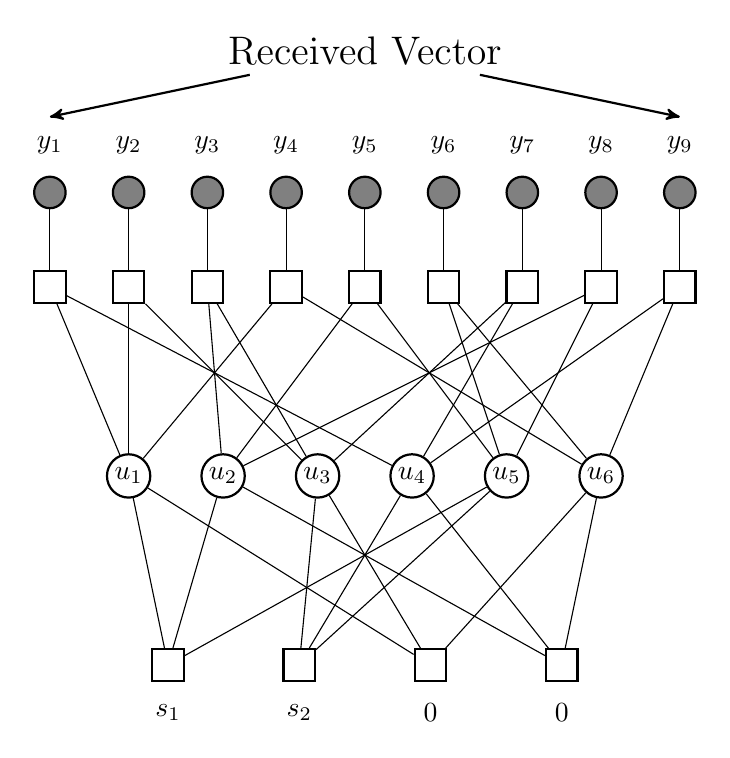
\begin{tikzpicture}
  [
  yscale=1.2,
  node distance = 12mm, draw=black, thick, >=stealth',
  bitnode/.style={circle, inner sep = 0pt, minimum size = 5.5mm, draw=black},
  checknode/.style={rectangle, inner sep = 0pt, minimum size = 4mm, draw=black},
  bitnode2/.style={circle, inner sep = 0pt, minimum size = 4mm, draw=black, fill=black!50},
  ]
  
  \node (rv) at (0,4.5) {\Large{Received Vector}};
  \draw[->] (rv) -- (-4,3.8);
  \draw[->] (rv) -- (4,3.8);

  \foreach \x in {1,2,...,9} {
    \node[bitnode2] (bb\x) at (\x-5,3) {};
  }

  \foreach \x in {1,2,...,9} {
    \node at (\x-5,3.5) {$y_{\x}$};
  }

  \foreach \x in {1,2,...,9} {
    \node[checknode] (c\x) at (\x-5,2) {};
    \draw[thin] (c\x) -- (bb\x);
  }

  \foreach \x in {1,2,...,6} {
    \node[bitnode] (b\x) at (1.2*\x-4.2,0) {$u_{\x}$};
  }

  \foreach \x in {1,...,4} {
    \node[checknode] (cc\x) at (5*\x/3-2.5-5/3,-2) {};
  }

  \draw[thin] (c1) -- (b4);
  \draw[thin] (c1) -- (b1);
  \draw[thin] (c2) -- (b1);
  \draw[thin] (c2) -- (b3);
  \draw[thin] (c3) -- (b3);
  \draw[thin] (c3) -- (b2);
  \draw[thin] (c4) -- (b1);
  \draw[thin] (c4) -- (b6);
  \draw[thin] (c5) -- (b2);
  \draw[thin] (c5) -- (b5);
  \draw[thin] (c6) -- (b5);
  \draw[thin] (c6) -- (b6);
  \draw[thin] (c7) -- (b3);
  \draw[thin] (c7) -- (b4);
  \draw[thin] (c8) -- (b5);
  \draw[thin] (c8) -- (b2);
  \draw[thin] (c9) -- (b4);
  \draw[thin] (c9) -- (b6);


  \draw[thin] (cc1) -- (b2);
  \draw[thin] (cc1) -- (b1);
  \draw[thin] (cc1) -- (b5);
  \draw[thin] (cc2) -- (b5);
  \draw[thin] (cc2) -- (b3);
  \draw[thin] (cc2) -- (b4);
  \draw[thin] (cc3) -- (b1);
  \draw[thin] (cc3) -- (b3);
  \draw[thin] (cc3) -- (b6);
  \draw[thin] (cc4) -- (b2);
  \draw[thin] (cc4) -- (b6);
  \draw[thin] (cc4) -- (b4);

  \node at (5*1/3-2.5-5/3,-2.5) {$s_1$};
  \node at (5*2/3-2.5-5/3,-2.5) {$s_2$};
  \node at (5*3/3-2.5-5/3,-2.5) {$0$};
  \node at (5*4/3-2.5-5/3,-2.5) {$0$};
\end{tikzpicture}

%%% Local Variables: 
%%% mode: latex
%%% TeX-master: "../talk"
%%% End: 
}

    \column{0.5\textwidth}
    \scalebox{0.5}{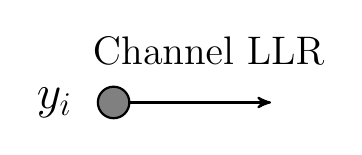
\begin{tikzpicture}
  [
  yscale=1.2,
  node distance = 12mm, draw=black, thick, >=stealth',
  bitnode/.style={circle, inner sep = 0pt, minimum size = 5.5mm, draw=black},
  checknode/.style={rectangle, inner sep = 0pt, minimum size = 4mm, draw=black},
  bitnode2/.style={circle, inner sep = 0pt, minimum size = 4mm, draw=black, fill=black!50},
  ]

  \node at (-0.75,0) {\LARGE{$y_i$}};
  \node[bitnode2] (vv1) at (0,0) {};
  
  \draw[->] (vv1) -- node[above,xshift=0.1cm,yshift=0.35cm]{\Large{Channel LLR}} (2,0);

\end{tikzpicture}


%%% Local Variables: 
%%% mode: latex
%%% TeX-master: "../talk"
%%% End: 
}\\ \vspace{0.3cm}
    \scalebox{0.5}{\input{Figures/mp_ldpc_bit}}\\ \vspace{0.3cm}
    \scalebox{0.5}{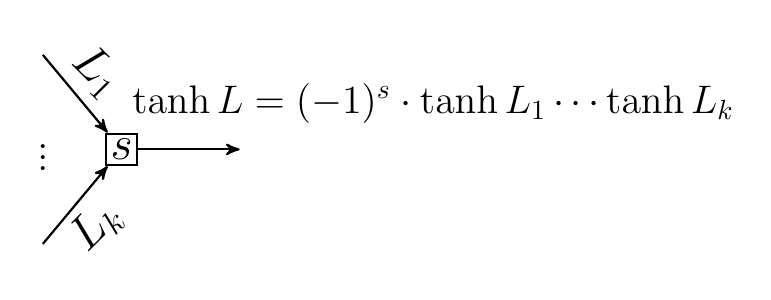
\begin{tikzpicture}
  [
  yscale=1.2,
  node distance = 12mm, draw=black, thick, >=stealth',
  bitnode/.style={circle, inner sep = 0pt, minimum size = 5.5mm, draw=black},
  checknode/.style={rectangle, inner sep = 0pt, minimum size = 4mm, draw=black},
  bitnode2/.style={circle, inner sep = 0pt, minimum size = 4mm, draw=black, fill=black!50},
  ]

  \node[checknode] (v1) at (0,0) {\LARGE{$s$}};
  
  \draw[->] (-1,1) -- node[midway,above,sloped]{\LARGE{$L_1$}} (v1);
  \node at (-1,0) {\LARGE{$\vdots$}};
  \draw[->] (-1,-1) -- node[midway,below,sloped]{\LARGE{$L_k$}} (v1);

  \draw[->] (v1) -- node[above,midway,xshift=3.1cm,yshift=0.2cm]{\Large{$\tanh L=(-1)^{s}\cdot \tanh L_1\cdots \tanh L_k$}} (1.5,0);

\end{tikzpicture}

%%% Local Variables: 
%%% mode: latex
%%% TeX-master: "../talk"
%%% End: 
}
  \end{columns}
  \begin{block}{Remarks}
    \begin{itemize}
    \item Standard message-passing algorithm
    \item Threshold saturation proven for SC compound codes on BEC
    \item Empirically observed for BMS channels
    \end{itemize}
  \end{block}
\end{frame}

\begin{frame}{Encoding in Spatially-Coupled Compound Codes}
  \begin{columns}
    \column{0.5\textwidth}
    \setlength\tikzheight{5cm}
    \setlength\tikzwidth{6cm}
    \scalebox{0.5}{\input{Figures/bpgd_compound_code}}

    \column{0.5\textwidth}
    \scalebox{0.5}{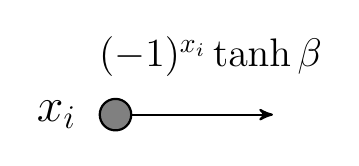
\begin{tikzpicture}
  [
  yscale=1.2,
  node distance = 12mm, draw=black, thick, >=stealth',
  bitnode/.style={circle, inner sep = 0pt, minimum size = 5.5mm, draw=black},
  checknode/.style={rectangle, inner sep = 0pt, minimum size = 4mm, draw=black},
  bitnode2/.style={circle, inner sep = 0pt, minimum size = 4mm, draw=black, fill=black!50},
  ]

  \node at (-0.75,0) {\LARGE{$x_i$}};
  \node[bitnode2] (vv1) at (0,0) {};
  
  \draw[->] (vv1) -- node[above,xshift=0.1cm,yshift=0.35cm]{\alert{\Large{$(-1)^{x_i} \tanh \beta$}}} (2,0);

\end{tikzpicture}


%%% Local Variables: 
%%% mode: latex
%%% TeX-master: "../talk"
%%% End: 
}\\ \vspace{0.3cm}
    \scalebox{0.5}{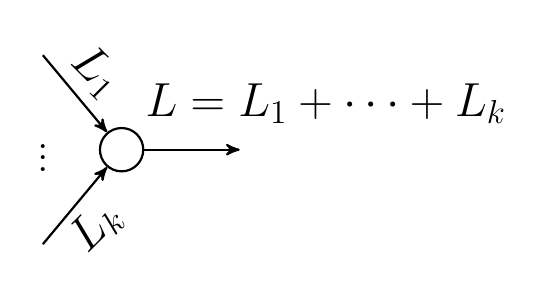
\begin{tikzpicture}
  [
  yscale=1.2,
  node distance = 12mm, draw=black, thick, >=stealth',
  bitnode/.style={circle, inner sep = 0pt, minimum size = 5.5mm, draw=black},
  checknode/.style={rectangle, inner sep = 0pt, minimum size = 4mm, draw=black},
  bitnode2/.style={circle, inner sep = 0pt, minimum size = 4mm, draw=black, fill=black!50},
  ]

  \node[bitnode] (v1) at (0,0) {};
  
  \draw[->] (-1,1) -- node[midway,above,sloped]{\LARGE{$L_1$}} (v1);
  \node at (-1,0) {\LARGE{$\vdots$}};
  \draw[->] (-1,-1) -- node[midway,below,sloped]{\LARGE{$L_k$}} (v1);

  \draw[->] (v1) -- node[above,midway,xshift=1.7cm,yshift=0.2cm]{\LARGE{$L=L_1+\cdots+L_k$}} (1.5,0);

\end{tikzpicture}

%%% Local Variables: 
%%% mode: latex
%%% TeX-master: "../talk"
%%% End: 
}\\ \vspace{0.3cm}
    \scalebox{0.5}{\input{Figures/bpgd_check}}
  \end{columns}
  \begin{block}{Remarks}
    \begin{itemize}
    \item \textcolor{blue}{Inverse temperature parameter $\beta$}
    \item Message-passing rules are the same
    \item However, a \alert{crucial decimation step is needed}
    \end{itemize}
  \end{block}
\end{frame}

\begin{frame}{Encoding in SC Compound Codes: BPGD Algorithm}
  \begin{algorithmic}
  \WHILE{\textcolor{blue}{There are active LDPC bit-nodes}}
    \FOR {\alert{$t=1$ to $T$}}
    \STATE Run the BP equations
    \ENDFOR
    \STATE Evaluate LLRs $m_{i}$ for each LDPC bit-node
    \STATE Choose max. of $|m_i|$ in \alert{left-most $w$ active sections}
    \IF{$|m_{i^*}|=0$}
    \STATE Set $u_{i^*}$ to $0$ or $1$ \textcolor{blue}{uniformly randomly}
    \ELSE
    \STATE Set $u_{i^*}$ to $0$ or $1$ with \alert{prob. $\frac{1+\tanh m_{i^*}}{2}$ or $\frac{1-\tanh m_{i^*}}{2}$}
    \ENDIF
    \STATE \alert{Decimate} (remove) LDPC bit-node $i^*$ and \textcolor{blue}{update parities}
    \ENDWHILE
    \STATE If $\{u_{i}\}$ fail to satisfy LDPC checks, then \textbf{\alert{re-encode}}
    %% Not an issue for lossy source coding problem
  \end{algorithmic}
\end{frame}

\begin{frame}{Encoding in SC Compound Codes: Remarks}
  \begin{itemize}
  \item \textcolor{blue}{Randomization} in setting $u_{i^*}$ is crucial \vspace{0.3cm}
  \item BPGD applied to uncoupled code \alert{always failed} \vspace{0.3cm}
  \item \alert{Spatially-coupled structure} is crucial for successful encoding \vspace{0.15cm}
    \begin{itemize}
    \item In addition, distortion is \textcolor{blue}{close to optimal thresholds} \vspace{0.2cm}
    \item \alert{Does not encode} if decimated from both \textcolor{blue}{left and right}\vspace{0.2cm}
    \item \alert{Does not encode} if both left and right boundary is set to 0 \vspace{0.2cm}
    \end{itemize}
  \end{itemize}
\end{frame}

\begin{frame}{Encoding in SC Compound Codes: Numerical Example}
  \begin{center}
    \begin{tabular}{|c|c|c|}
      \hline
      Block length ($n$) & 4-cycles & Attempts $1/2/3/4/\geq 5$  \\
      \hline
      \textcolor{blue}{$9000$} & \textcolor{blue}{yes} & \textcolor{blue}{$5/3/5/2/35$} \\
      $9000$ & no & $21/12/5/3/9$ \\
      $27000$ & no & $35/15/0/0/0$ \\
      $45000$ & no & $40/9/0/0/1$ \\
      $63000$ & no & $44/6/0/0/0$ \\
      \alert{$81000$} & \alert{no} & \alert{$50/0/0/0/0$}\\ 
      \hline  
    \end{tabular}
  \end{center}
  \begin{block}{Remarks}
    \begin{itemize}
    \item \# Attempts to encode $50$ seq.~in $(6,3)$ LDGM / $(3,6)$ LDPC
    \item $L=20$, $w=4$, $\beta=0.65$, $T=10$
    \item Removing \alert{4-cycles} dramatically improves success
    \item How much do \textcolor{blue}{6-cycles} matter?
    \end{itemize}
  \end{block}
\end{frame}

\begin{frame}{Numerical Results: Wyner-Ziv}
  \begin{center}
    \begin{tabular}{|c|c|c|c|c|}
      \hline
      LDGM & LDPC & $(L,w)$ & $(D_{*},\delta_{*})$ & $(D,\delta)$ \\
      $(d_v,d_c)$ & $(d'_v,d'_c)$ &  &  & \\
      \hline
      $(6,3)$ & (3,6) & (20,4)  & (0.111,0.134)  & (0.1174,0.122) \\
      $(8,4)$ & (3,6) & (20,4)  & (0.111,0.134)  & (0.1149,0.120) \\
      $(10,5)$ & (3,6) & (20,4)  & (0.111,0.134)  & (0.1139,0.122) \\
      \hline  
    \end{tabular}
  \end{center}
  \begin{block}{Remarks}
    \begin{itemize}
    \item $D_*$ and $\delta_*$ are calculated based on the rate of the respective code:
      \begin{align*}
        D_*&=h^{-1}(1-R1)  & \delta_*&=h^{-1}(1-R2)
      \end{align*}
    \item $n\approx 140000$, $\beta=1.04$, $T=10$
    \end{itemize}
  \end{block}
\end{frame}

\begin{frame}{Numerical Results: Gelfand-Pinsker}
  \begin{center}
    \begin{tabular}{|c|c|c|c|c|}
      \hline
      LDGM & LDPC & $(L,w)$ & $(p_{*},\delta_{*})$ & $(p,\delta)$ \\
      $(d_v,d_c)$ & $(d'_v,d'_c)$ &  &  & \\
      \hline
      $(6,3)$ & (3,6) & (20,4)  & (0.215,0.157)  & (0.2200,0.152) \\
      $(8,4)$ & (3,6) & (20,4)  & (0.215,0.157)  & (0.2230,0.151) \\
      $(10,5)$ & (3,6) & (20,4)  & (0.215,0.157)  & (0.2200,0.151) \\
      \hline
    \end{tabular}
  \end{center}
  \begin{block}{Remarks}
    \begin{itemize}
    \item $p_*$ and $\delta_*$ are calculated based on the rate of the respective code:
      \begin{align*}
        p_*&=h^{-1}(1-R1)  & \delta_*&=h^{-1}(1-R2)
      \end{align*}
    \item $n\approx 140000$, $\beta=0.65$, $T=10$
    \end{itemize}
  \end{block}
\end{frame}

\begin{frame}{Concluding Remarks}
  \begin{block}{Conclusion}
    \begin{itemize}
    \item Spatially-coupled codes achieve the rate regions of Wyner-Ziv and Gelfand-Pinsker problems \vspace{0.2cm}
    \item \textcolor{red}{Coupling structure} is also crucial 
      \begin{itemize}
      \item to achieve optimum thresholds
      \item for encoding to succeed with decimation 
      \end{itemize}
    \end{itemize}
  \end{block}
  \begin{block}{Open Questions}
    \begin{itemize}
    \item Effect of degree profiles, short-cycles on encoding success \vspace{0.2cm}
    \item Precise trade-offs with \textcolor{blue}{polar codes}
    \end{itemize}
  \end{block}
\end{frame}

\end{document}
